\subsection[\englishfont 2.1 基于分层车联网架构的车载信息物理融合质量指标设计与优化]{2.1 基于分层车联网架构的车载信息物理融合质量指标设计与优化}

\begin{frame}{研究贡献}
\newBackground
\begin{center}
\begin{textblock*}{\textwidth}(-1cm,1.8cm)
  \small \englishfont \colorbox{cqublue}{\color{white}{创新的服务架构和高效的数据感知与质量}}
\end{textblock*}
\end{center}

\begin{center}
\begin{textblock*}{\textwidth}(-1cm,2.3cm)
  \small \englishfont \colorbox{cqublue}{\color{white}{评估模型是 VCPS的{\color{yellow}{架构基础}}与{\color{yellow}{驱动核心}}}}
\end{textblock*}
\end{center}

\begin{center}
\begin{textblock*}{\textwidth}(-1.8cm,3.16cm)
\begin{minipage}[t]{0.7\textwidth}
\begin{itemize}[itemsep=0.2\baselineskip] \englishfont
	\item[\ding{111}] {{\color{cqublue}{\textbf{架构}}}:{\color{red}{SDN+MEC}}车联网分层架构}
	\item[\ding{111}]  {{\color{cqublue}{\textbf{指标}}}:{\color{red}{Age of View}}评估逻辑视图质量}
		\begin{itemize}[itemsep=0.2\baselineskip] 
		\begin{small}
		\item[\ding{226}] 时效性、完整性、一致性
		\item[\ding{226}] 最大化VCPS质量问题
		\end{small}
		\end{itemize}
	\item[\ding{111}]  {{\color{cqublue}{\textbf{算法}}}:基于差分奖励的多智能体强化学习 ({\color{red}{MADR}})}
	\item[\ding{111}]  {{\color{cqublue}{\textbf{实验}}}:有效提高车载信息物理融合质量}
\end{itemize}
\end{minipage}
\end{textblock*}
\end{center}

\begin{center}
\begin{textblock*}{\textwidth}(-1cm,6.7cm)
\fbox{\begin{minipage}[t]{0.78\textwidth}\englishfont \tiny [1] LIU K, \underline{\textcolor{cqublue}{\textbf{XU X}}},  et al. \textcolor{cqublue}{A hierarchical architecture for the future Internet of Vehicles}[J].IEEE Communications Magazine (\textcolor{red}{ComMag}), 2019, 57(7): 41-47. 影响因子: 9.03(2021), 10.892(5年) (中科院SCI 1区)
\end{minipage}}
\fbox{\begin{minipage}[t]{0.78\textwidth}\englishfont \tiny [2] \underline{\textcolor{cqublue}{\textbf{XU X}}}, LIU K, et al. \textcolor{cqublue}{Cooperative sensing and heterogeneous information fusion in VCPS: A multi-agent deep reinforcement learning approach}[J]. IEEE Transactions on Intelligent Transportation Systems (\textcolor{red}{T-ITS}), under major revision. (中科院SCI 1区)
\end{minipage}}
\end{textblock*}
\end{center}

\begin{center}
\begin{textblock*}{\textwidth}(7cm,1.8cm)
\begin{figure}
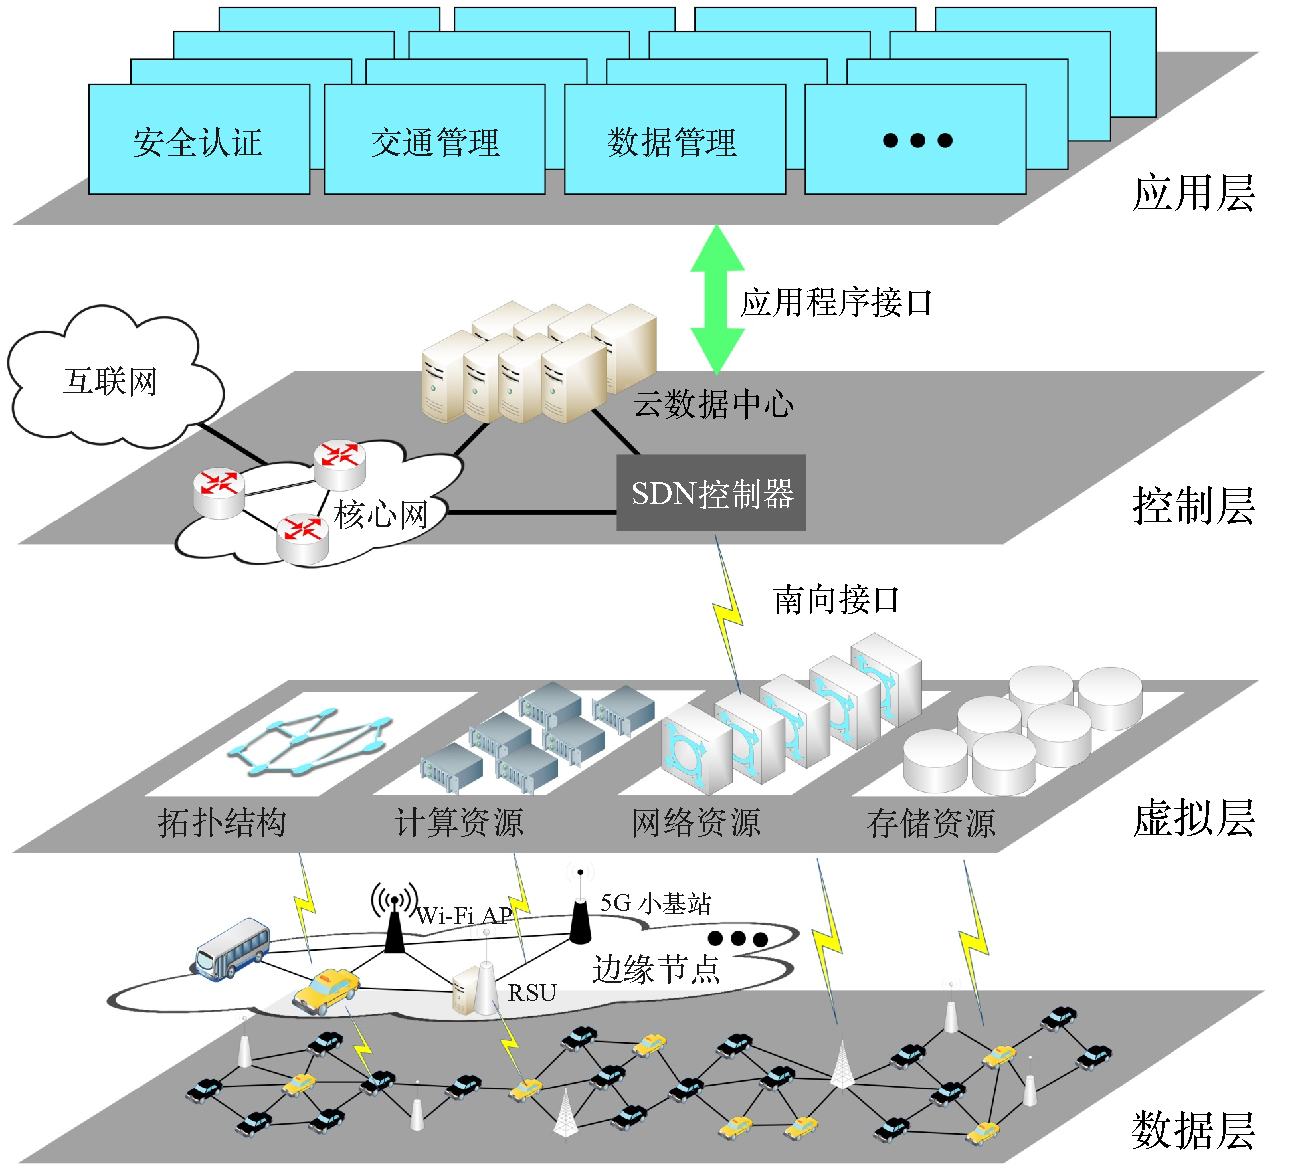
\includegraphics[width=0.23\textwidth]{fig/Fig2-1-hierarchical-architecture.pdf}
\end{figure}
\begin{figure}
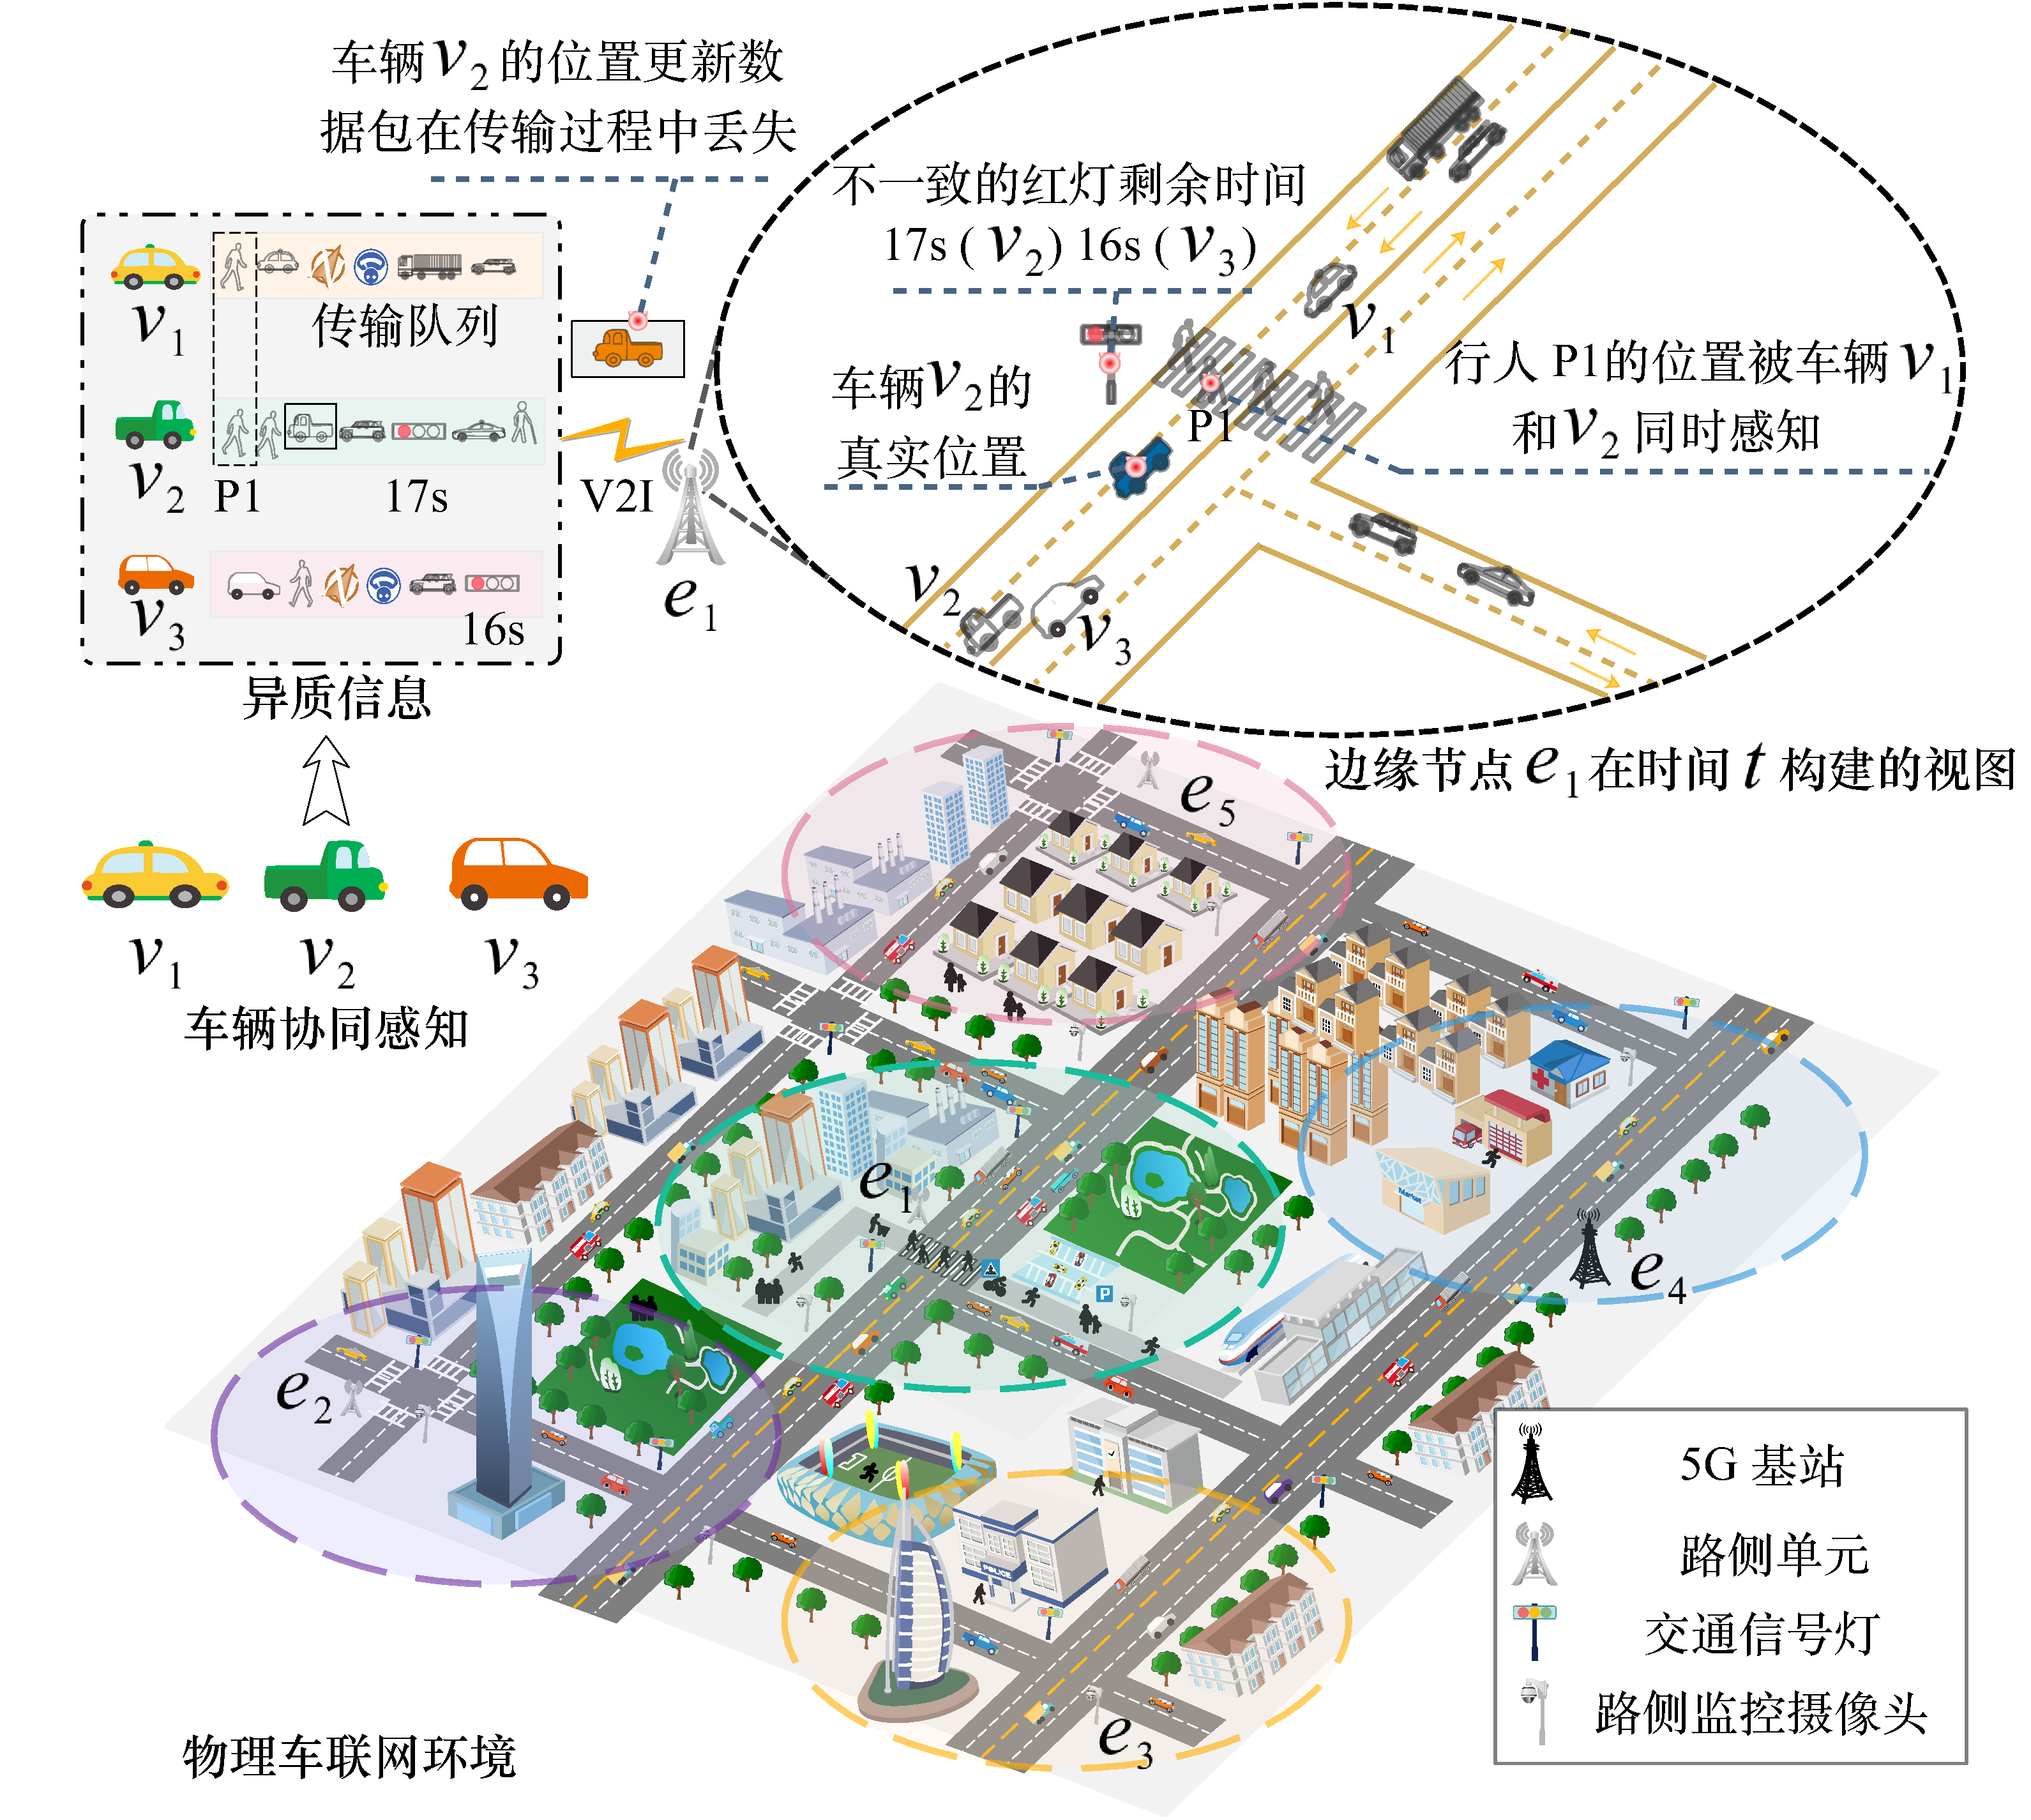
\includegraphics[width=0.23\textwidth]{fig/Fig2-2a-architerture.pdf}
\end{figure}
\end{textblock*}
\end{center}
\end{frame}

\begin{frame}
\frametitle{\englishfont \underline{架构}:车联网分层服务架构}
\newBackground
\begin{center}
\begin{textblock*}{\textwidth}(0.5cm,2.5cm)
\begin{itemize}[itemsep=0.2\baselineskip]  \englishfont
	\item[\ding{111}] {\color{cqublue}{{软件定义网络 ({\color{cqublue}{SDN}})+移动边缘计算 ({\color{cqublue}{MEC}})}}}
	\begin{itemize}[itemsep=0.2\baselineskip] 
	\begin{small}
		\item[\ding{226}] SDN逻辑上集中控制
		\item[\ding{226}] MEC分布式服务
	\end{small}
	\end{itemize}
	\item[\ding{111}]  {\color{cqublue}{分层服务架构}}
	\begin{itemize}[itemsep=0.2\baselineskip] 
	\begin{small}
		\item[\ding{226}] \underline{应用层}:面向业务需求的应用
		\item[\ding{226}] \underline{控制层}:网络功能集中控制
		\item[\ding{226}] \underline{虚拟层}:抽象计算、网络和存储资源
		\item[\ding{226}] \underline{数据层}:存储、处理数据
		\item 
	\end{small} 
	\end{itemize}
\end{itemize}
\end{textblock*}
\end{center}

\begin{center}
\begin{textblock*}{\textwidth}(5.2cm,1.8cm)
\begin{figure}
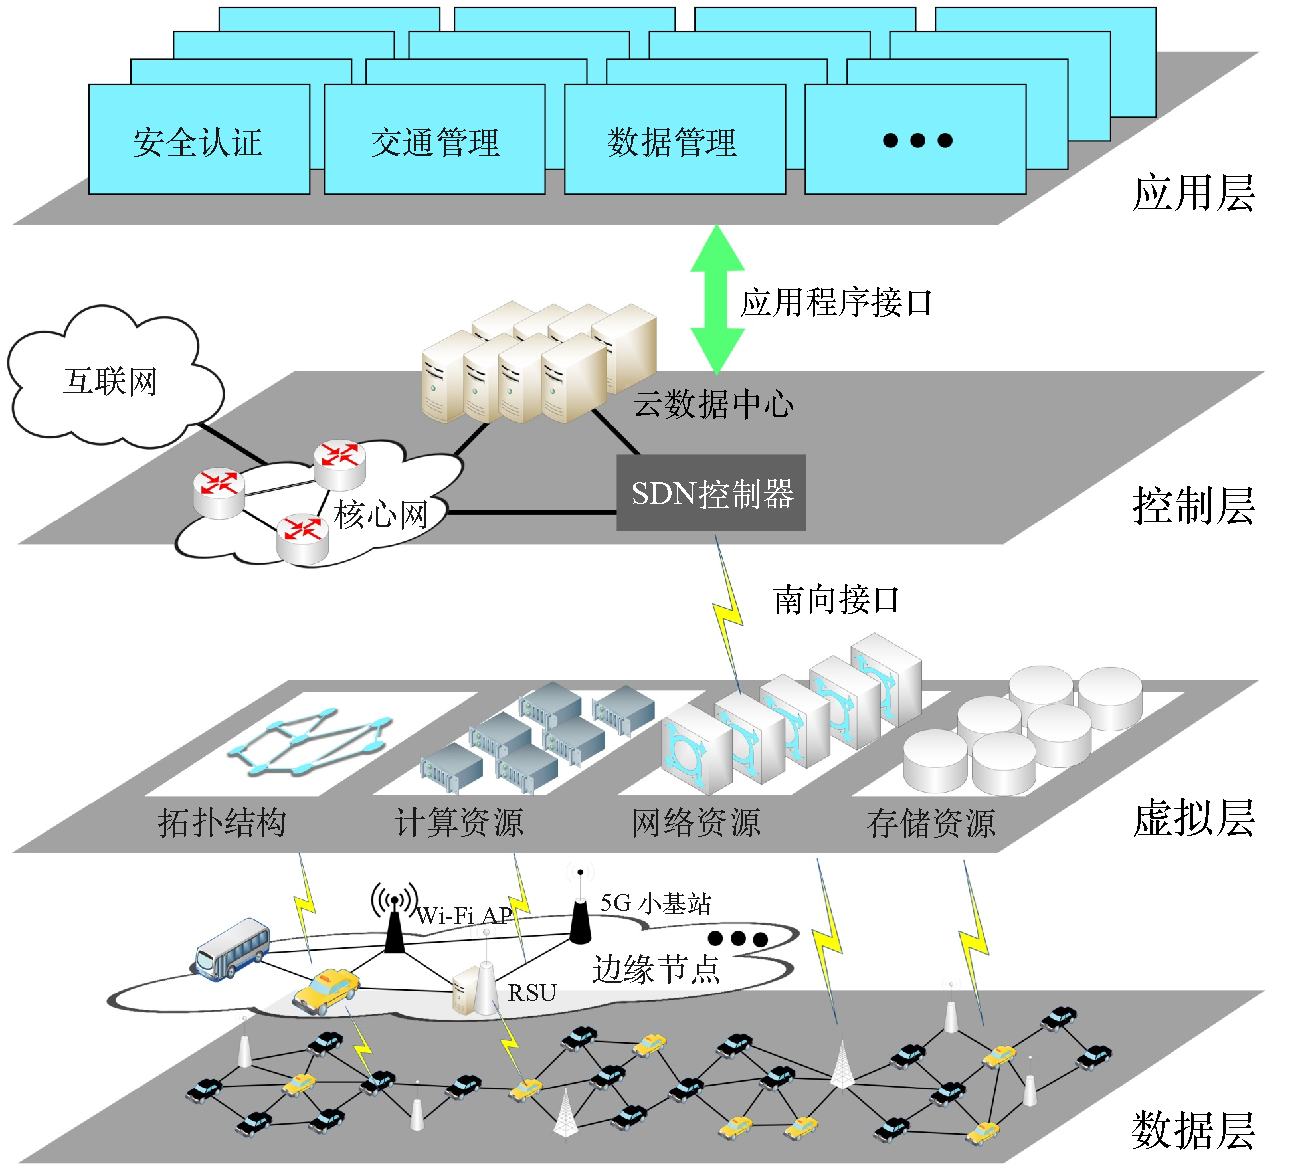
\includegraphics[width=0.47\textwidth]{fig/Fig2-1-hierarchical-architecture.pdf}
\end{figure}
\end{textblock*}
\end{center}
\end{frame}

\begin{frame}
\frametitle{\underline{指标}:感知与信息融合场景}
\newBackground
\begin{center}
\begin{textblock*}{\textwidth}(5.2cm,1.8cm)
\begin{figure}
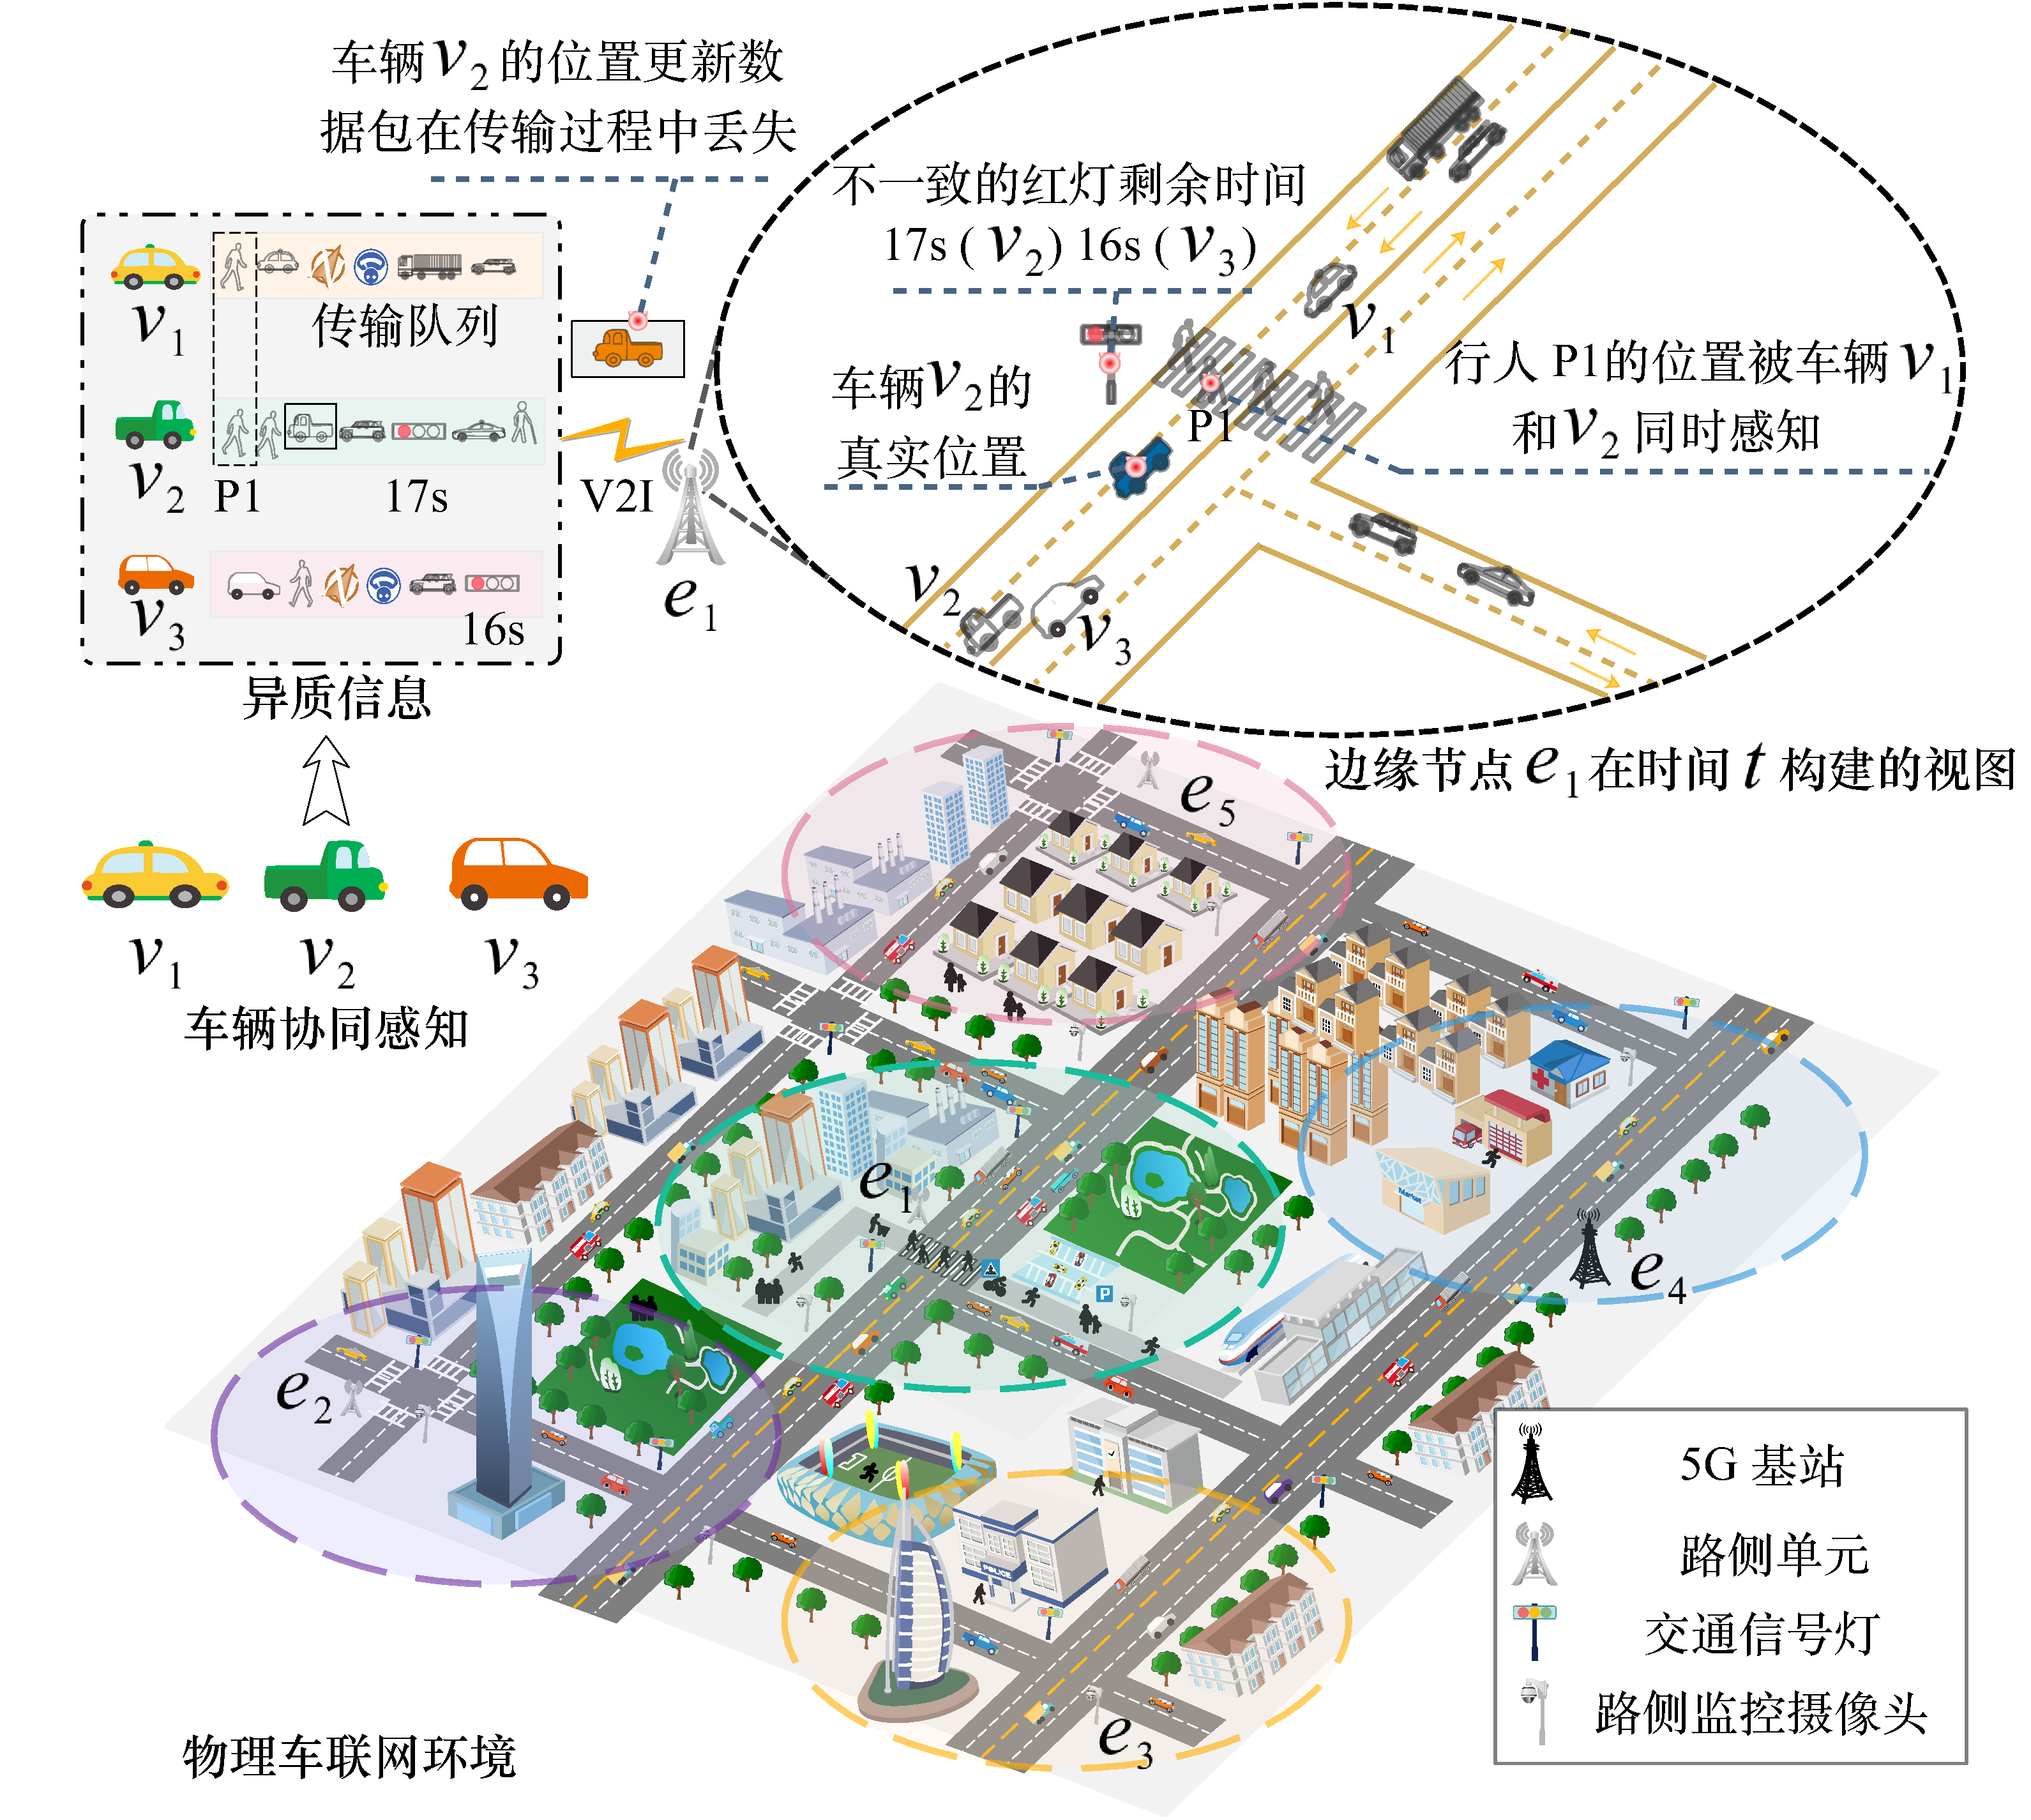
\includegraphics[width=0.47\textwidth]{fig/Fig2-2a-architerture.pdf}
\end{figure}
\end{textblock*}
\end{center}

\begin{center}
\begin{textblock*}{\textwidth}(0.5cm,2.1cm)
\begin{itemize}[itemsep=0.2\baselineskip]  \englishfont
	\item[\ding{111}] {\color{cqublue}{工作流程}}
	\begin{itemize}[itemsep=0.2\baselineskip] 
	\begin{small}
		\item[\ding{226}] \underline{感知}:感知频率、上传优先级
		\item[\ding{226}] \underline{上传}:V2I带宽
		\item[\ding{226}] \underline{视图构建}:信息融合,支撑 ITS 应用
	\end{small}
	\end{itemize}
	\item[\ding{111}]  {\color{cqublue}{速度建议应用为例}}
	\begin{itemize}[itemsep=0.2\baselineskip] 
	\begin{small}
		\item[\ding{226}] 信息不一致
			\begin{itemize}[itemsep=0.2\baselineskip]  \footnotesize
				\item[\ding{61}] 红灯剩余时间 {\color{cqublue}{17s}} (车辆$v_2$) {\color{cqublue}{16s}} (车辆$v_3$)
			\end{itemize}
		\item[\ding{226}] 重复感知
		\begin{itemize}[itemsep=0.2\baselineskip]  \footnotesize
			\item[\ding{61}] 同一物理要素的状态被多车感知
		\end{itemize}
		\item[\ding{226}] 物理环境与视图的差异
			\begin{itemize} [itemsep=0.2\baselineskip] \footnotesize
				\item[\ding{61}]数据包丢失 (车辆$v_2$的位置)
			\end{itemize}
		\item 
	\end{small} 
	\end{itemize}
\end{itemize}
\end{textblock*}
\end{center}
\end{frame}

\begin{frame}
\frametitle{\englishfont \underline{指标}:协同感知模型}
\newBackground
\begin{center}
\begin{textblock*}{\textwidth}(5.2cm,2.2cm)
\begin{figure}
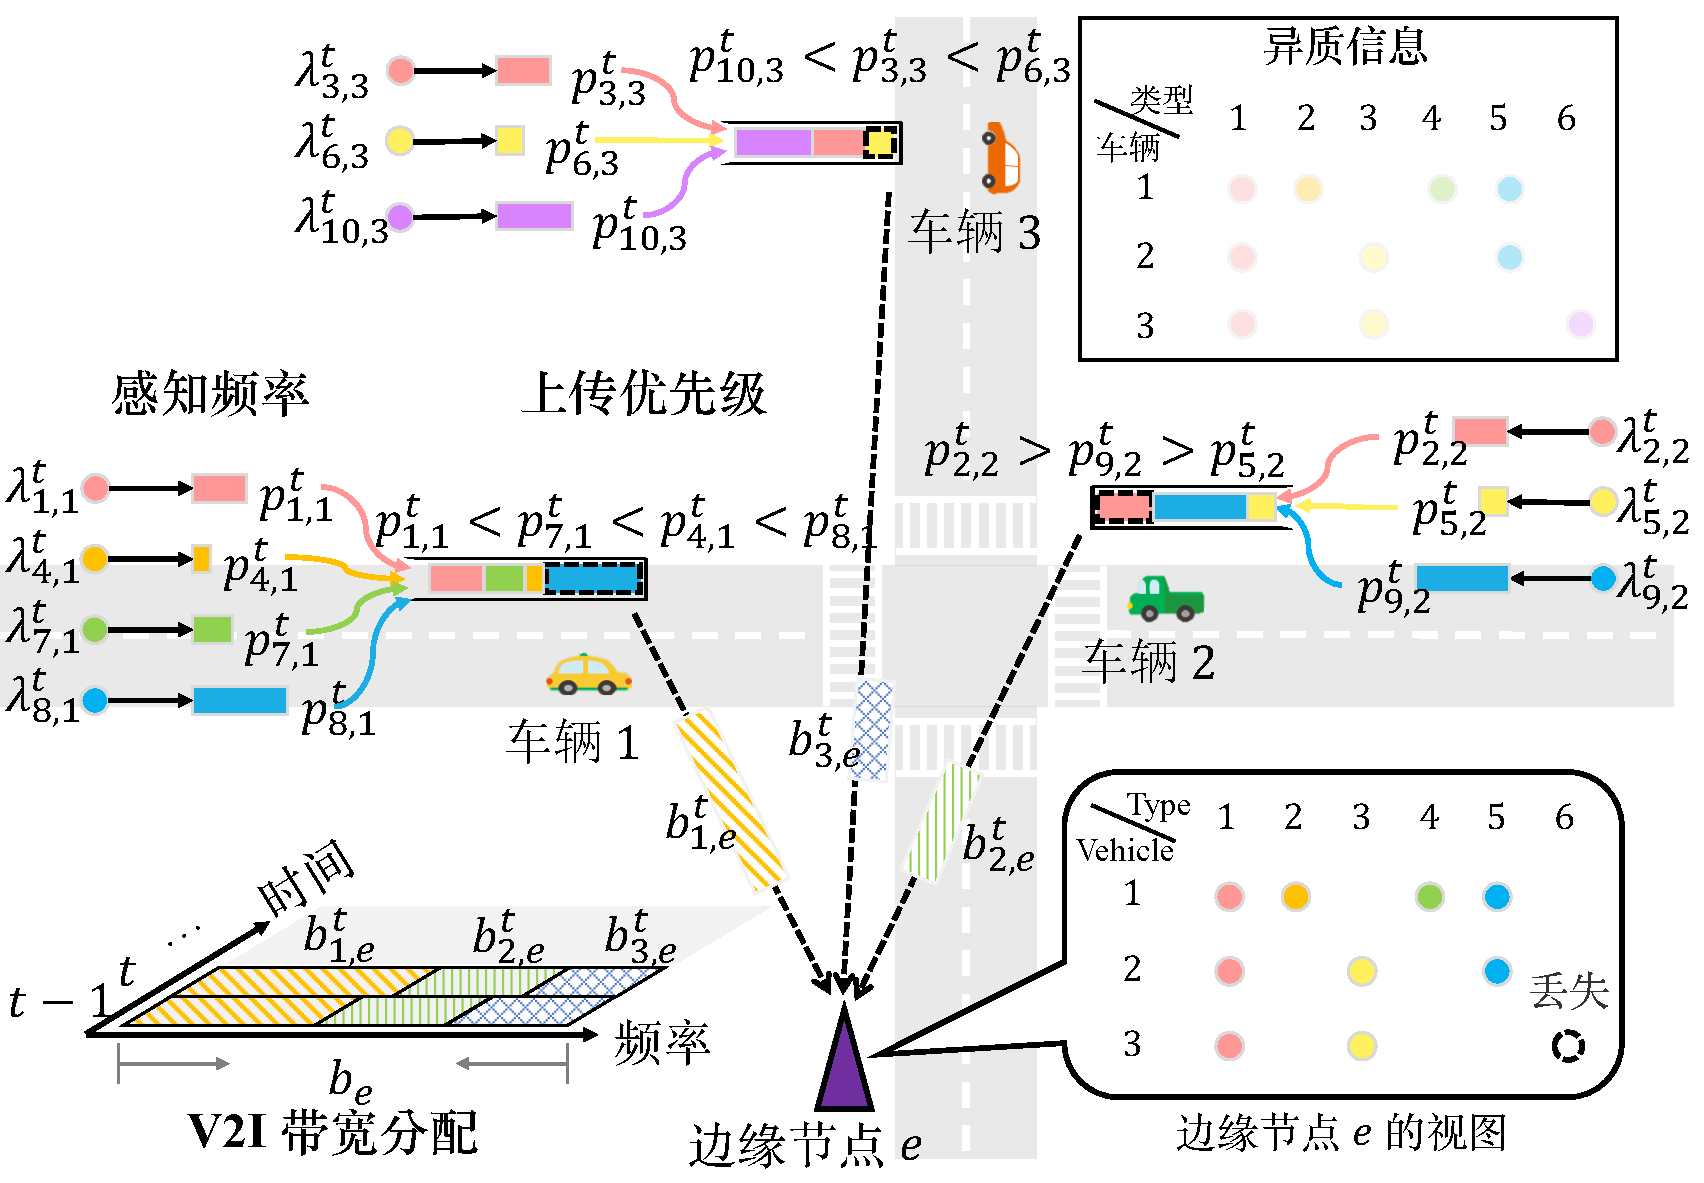
\includegraphics[width=0.55\textwidth]{fig/Fig2-3-cooperative-sensing.pdf}
\end{figure}
\end{textblock*}
\end{center}

% 添加动画效果

\begin{overlayarea}{\textwidth}{3cm}
\only<1-2>{
\begin{center}
\begin{textblock*}{1\textwidth}(-2cm,2.0cm)
\footnotesize
\begin{equation}
	\operatorname{\bar{q}}_{d, v}^t= \frac{1} {1 - \rho_{d, v}^{t}} 
        \left[ \alpha_{d, v}^t + \frac{ \lambda_{d, v}^{t} \beta_{d, v}^t + \sum\limits_{\forall d^* \in \mathbf{D}_{d, v}^t} \lambda_{d^*,s}^t \beta_{d^*, v}^t }{2\left(1-\rho_{d, v}^{t} - \lambda_{d, v}^{t}  \alpha_{d, v}^t\right)}\right] 
        - \alpha_{d, v}^t \notag
\end{equation}
\end{textblock*}
\end{center}
}

\only<2->{%
\begin{center}
\begin{textblock*}{1\textwidth}(-2cm,2.0cm)
\footnotesize
\begin{equation}
	\operatorname{\bar{q}}_{d, v}^t= \frac{1} {1 - \rho_{d, v}^{t}} 
        \left[ \alpha_{d, v}^t + \frac{ {\color{red}{ \lambda_{d, v}^{t} }}\beta_{d, v}^t + \sum\limits_{\forall d^* \in \mathbf{D}_{d, v}^t} \lambda_{d^*,s}^t \beta_{d^*, v}^t }{2\left(1-\rho_{d, v}^{t} - \lambda_{d, v}^{t}  \alpha_{d, v}^t\right)}\right] 
        - \alpha_{d, v}^t \notag
\end{equation}
\end{textblock*}
\end{center}
}

\only<3-4>{
\begin{center}
\begin{textblock*}{1\textwidth}(-3cm,4.9cm)
\footnotesize
\begin{equation}
\mathrm{w}_{d, v, e}^t=\frac{\left|d\right|}{b_{v, e}^{t} \log _{2}\left(1+\mathrm{SNR}_{v, e}^{t}\right)} \notag
\end{equation}
\end{textblock*}
\end{center}
}
\only<4->{
\begin{center}
\begin{textblock*}{1\textwidth}(-3cm,4.9cm)
\footnotesize
\begin{equation}
\mathrm{w}_{d, v, e}^t=\frac{\left|d\right|}{{\color{red}{b_{v, e}^{t}}} \log _{2}\left(1+\mathrm{SNR}_{v, e}^{t}\right)} \notag
\end{equation}
\end{textblock*}
\end{center}
}
\end{overlayarea}

\begin{center}
\begin{textblock*}{0.6\textwidth}(0.5cm,1.8cm)
\begin{itemize} \englishfont
	\item[\ding{111}]  {\color{cqublue}{排队时间}}
	\item 
	\item
	\item
	\item<2-> {\small{{\color{red}{ $\lambda_{d, v}^{t}$ }}:信息感知频率}}
	\item<3->[\ding{111}] {\color{cqublue}{传输时间}}
	\item
	\item 
	\item<4-> {\color{red}{$b_{v, e}^{t}$}}:V2I带宽
	\item<5->[\ding{111}] {\color{cqublue}{传输成功与否}}
		\begin{itemize}
		\begin{small}
			\item[\ding{226}] $\mathrm{SNR}_{\text {wall }}=\frac{\sigma^{2}-1}{\sigma}$
		\end{small}
	\end{itemize}
\end{itemize}
\end{textblock*}
\end{center}
\end{frame}

\begin{frame}{车载信息物理融合质量指标设计}
\frametitle{\englishfont \underline{指标}:Age of View}
\newBackground
\begin{overlayarea}{\textwidth}{3cm}
\only<1-1>{
\begin{center}
\begin{textblock*}{1\textwidth}(-3cm,1.8cm)
\begin{equation}
\Xi_{i}= \sum_{\forall v \in \mathbf{V}} \sum_{\forall d \in \mathbf{D}_{i, e} \cap \mathbf{D}_v^t } \xi_{d, v} \notag
\end{equation}
\end{textblock*}
\end{center}
}

\only<2-2>{
\begin{center}
\begin{textblock*}{1\textwidth}(-3cm,1.8cm)
\begin{equation}
\Xi_{i}= \sum_{\forall v \in \mathbf{V}} \sum_{\forall d \in \mathbf{D}_{i, e} \cap \mathbf{D}_v^t } {\color{red}{ \xi_{d, v}}} \notag
\end{equation}
\end{textblock*}
\end{center}
}

\only<3->{
\begin{center}
\begin{textblock*}{1\textwidth}(-3cm,1.8cm)
\begin{equation}
\Xi_{i}= \sum_{\forall v \in \mathbf{V}} \sum_{\forall d \in \mathbf{D}_{i, e} \cap \mathbf{D}_v^t }  \xi_{d, v} \notag
\end{equation}
\end{textblock*}
\end{center}
}

\only<2-2>{
\begin{center}
\begin{textblock*}{1\textwidth}(2cm,1.8cm)
\begin{equation}
{\color{red}{\xi_{d,v}}} = \operatorname{a}_{d, v}^t + \operatorname{q}_{d, v}^t + \operatorname{w}_{d, v, e}^t \notag
\end{equation}
\end{textblock*}
\end{center}
}
\only<3-3>{
\begin{center}
\begin{textblock*}{1\textwidth}(2cm,1.8cm)
\begin{equation}
\xi_{d,v} = {\color{red}{\operatorname{a}_{d, v}^t}} + \operatorname{q}_{d, v}^t + \operatorname{w}_{d, v, e}^t \notag
\end{equation}
\end{textblock*}
\end{center}
}

\only<3-3>{
\begin{center}
\begin{textblock*}{1\textwidth}(1.7cm,3.1cm)
\small
{\color{red}{$\operatorname{a}_{d, v}^t$}}:间隔到达时间
\end{textblock*}
\end{center}
}

\only<4-4>{
\begin{center}
\begin{textblock*}{1\textwidth}(2cm,1.8cm)
\begin{equation}
\xi_{d,v} = \operatorname{a}_{d, v}^t + {\color{red}{\operatorname{q}_{d, v}^t}} + \operatorname{w}_{d, v, e}^t \notag
\end{equation}
\end{textblock*}
\end{center}
}

\only<4-4>{
\begin{center}
\begin{textblock*}{1\textwidth}(1.7cm,3.1cm)
\small
{\color{red}{$\operatorname{q}_{d, v}^t$}}:排队时间
\end{textblock*}
\end{center}
}

\only<5-5>{
\begin{center}
\begin{textblock*}{1\textwidth}(2cm,1.8cm)
\begin{equation}
\xi_{d,v} = \operatorname{a}_{d, v}^t + \operatorname{q}_{d, v}^t + {\color{red}{\operatorname{w}_{d, v, e}^t}} \notag
\end{equation}
\end{textblock*}
\end{center}
}

\only<5-5>{
\begin{center}
\begin{textblock*}{1\textwidth}(1.7cm,3.1cm)
\small
{\color{red}{$\operatorname{w}_{d, v, e}^t$}}:传输时间
\end{textblock*}
\end{center}
}

\only<6->{
\begin{center}
\begin{textblock*}{1\textwidth}(2cm,1.8cm)
\begin{equation}
\xi_{d,v} = \operatorname{a}_{d, v}^t + \operatorname{q}_{d, v}^t + \operatorname{w}_{d, v, e}^t \notag
\end{equation}
\end{textblock*}
\end{center}
}

\only<1-5>{
\begin{center}
\begin{textblock*}{1\textwidth}(-3.6cm,3.6cm)
\begin{equation}
\Phi_{i} = {| \mathbf{D}_{i, e} |} \big/ {|D_{i} |} \notag
\end{equation}
\end{textblock*}
\end{center}
}

\only<6-6>{
\begin{center}
\begin{textblock*}{1\textwidth}(-3.6cm,3.6cm)
\begin{equation}
\Phi_{i} = {{\color{red}{| \mathbf{D}_{i, e} |}}} \big/ {|D_{i} |} \notag
\end{equation}
\end{textblock*}
\end{center}
}

\only<6-6>{
\begin{center}
\begin{textblock*}{1\textwidth}(1.5cm,4.2cm)
\small
{\color{red}{${| \mathbf{D}_{i, e} |}$}}:收到信息数量
\end{textblock*}
\end{center}
}

\only<7-7>{
\begin{center}
\begin{textblock*}{1\textwidth}(-3.6cm,3.6cm)
\begin{equation}
\Phi_{i} = {| \mathbf{D}_{i, e} |} \big/ {{\color{red}{|D_{i} |}}} \notag
\end{equation}
\end{textblock*}
\end{center}
}

\only<7-7>{
\begin{center}
\begin{textblock*}{1\textwidth}(1.5cm,4.2cm)
\small
{\color{red}{$|D_{i} |$}}:所需信息总量
\end{textblock*}
\end{center}
}

\only<8->{
\begin{center}
\begin{textblock*}{1\textwidth}(-3.6cm,3.6cm)
\begin{equation}
\Phi_{i} = {| \mathbf{D}_{i, e} |} \big/ {|D_{i} |} \notag
\end{equation}
\end{textblock*}
\end{center}
}

\only<1-7>{
\begin{center}
\begin{textblock*}{1\textwidth}(-1.7cm,4.8cm)
\begin{equation}
\Psi_{i}=\sum_{\forall v \in \mathbf{V}} \sum_{\forall d \in \mathbf{D}_{i, e} \cap \mathbf{D}_v^t} \left|\operatorname{q}_{d, v}^t + \operatorname{w}_{d, v, e}^t - \psi_{i} \right|^{2} \notag
\end{equation}
\end{textblock*}
\end{center}
}

\only<8-8>{
\begin{center}
\begin{textblock*}{1\textwidth}(-1.7cm,4.8cm)
\begin{equation}
\Psi_{i}=\sum_{\forall v \in \mathbf{V}} \sum_{\forall d \in \mathbf{D}_{i, e} \cap \mathbf{D}_v^t} \left| {\color{red}{\operatorname{q}_{d, v}^t + \operatorname{w}_{d, v, e}^t}} - \psi_{i} \right|^{2} \notag
\end{equation}
\end{textblock*}
\end{center}
}

\only<8-8>{
\begin{center}
\begin{textblock*}{1\textwidth}(5cm,5.4cm)
\small
{\color{red}{$\operatorname{q}_{d, v}^t + \operatorname{w}_{d, v, e}^t$}}:信息接收时间
\end{textblock*}
\end{center}
}

\only<9-9>{
\begin{center}
\begin{textblock*}{1\textwidth}(-1.7cm,4.8cm)
\begin{equation}
\Psi_{i}=\sum_{\forall v \in \mathbf{V}} \sum_{\forall d \in \mathbf{D}_{i, e} \cap \mathbf{D}_v^t} \left|\operatorname{q}_{d, v}^t + \operatorname{w}_{d, v, e}^t - {\color{red}{\psi_{i}}}\right|^{2} \notag
\end{equation}
\end{textblock*}
\end{center}
}

\only<9-9>{
\begin{center}
\begin{textblock*}{1\textwidth}(4cm,5.4cm)
\small
{\color{red}{$\psi_{i}$}}:平均接收时间
\end{textblock*}
\end{center}
}

\only<10->{
\begin{center}
\begin{textblock*}{1\textwidth}(-1.7cm,4.8cm)
\begin{equation}
\Psi_{i}=\sum_{\forall v \in \mathbf{V}} \sum_{\forall d \in \mathbf{D}_{i, e} \cap \mathbf{D}_v^t} \left|\operatorname{q}_{d, v}^t + \operatorname{w}_{d, v, e}^t - \psi_{i} \right|^{2} \notag
\end{equation}
\end{textblock*}
\end{center}
}
\end{overlayarea}


\begin{center}
\begin{textblock*}{1\textwidth}(1cm,1.8cm)
\begin{itemize} \englishfont
	\item[\ding{111}] {\color{cqublue}{时效性}}
	\item
	\item
	\item[\ding{111}]  {\color{cqublue}{完整性}}
	\item
	\item[\ding{111}]  {\color{cqublue}{一致性}}
	\item
	\item
	\item<10->[\ding{111}]  {\color{cqublue}{Age of View}}
	\begin{itemize}
	\begin{small}
		\item[\ding{226}] 归一化时效性、完整性和一致性的加权平均值
		\item[\ding{226}] $\operatorname{AoV}_{i} = w_1  \hat{\Xi}_{i} + w_2  \hat{\Phi}_{i}+  w_3 \hat{\Psi}_{i}$
	\end{small}
	\end{itemize}
\end{itemize}
\end{textblock*}
\end{center}
\end{frame}

\begin{frame}
\frametitle{\englishfont \underline{指标}:最大化VCPS质量问题}
\newBackground

\begin{overlayarea}{\textwidth}{3cm}
\only<1-1>{
\begin{center}
\begin{textblock*}{1\textwidth}(0.5cm,1.6cm)
\begin{align}
	\mathcal{P}2.1: &\max_{\boldsymbol{\Lambda}, \mathbf{P}, \mathbf{B}} \Upsilon \notag \\
	\text { s.t. }
    \mathcal{C}2.1: & \lambda_{d,v}^{t} \in \left [\lambda_{d,v}^{\min} , \lambda_{d,v}^{\max} \right ], \forall d \in \mathbf{D}_v^t , \forall v \in \mathbf{V}, \forall t \in \mathbf{T} \notag \\
     \mathcal{C}2.2: &{p}_{d^*, v}^t \neq {p}_{d, v}^t, \forall d^* \in \mathbf{D}_v^t \backslash \left\{ d\right \}, \forall d \in \mathbf{D}_v^t, \forall v \in \mathbf{V} \notag \\
    \mathcal{C}2.3: & b_{v, e}^t \in \left[ 0 , b_e \right ], \forall v \in \mathbf{V}_e^t, \forall e \in \mathbf{E}, \forall t \in \mathbf{T} \notag \\
    \mathcal{C}2.4: & \sum_{\forall d \subseteq \mathbf{D}_v^t} \lambda_{d,v}^{t}  \alpha_{d, v}^t < 1,\ \forall v \in \mathbf{V}, \forall t \in \mathbf{T}  \notag \\
    \mathcal{C}2.5: & {\sum_{\forall v \in \mathbf{V}_e^{t}}b_{v, e}^t} \leq b_e, \forall e \in \mathbf{E}, \forall t \in \mathbf{T} \notag
\end{align}	
\end{textblock*}
\end{center}
}

\only<2-2>{
\begin{center}
\begin{textblock*}{1\textwidth}(0.5cm,1.6cm)
\begin{align}
	\mathcal{P}2.1: &\max_{\boldsymbol{\Lambda}, \mathbf{P}, \mathbf{B}} {\color{red}{\Upsilon}} \notag \\
	\text { s.t. }
    \mathcal{C}2.1: & \lambda_{d,v}^{t} \in \left [\lambda_{d,v}^{\min} , \lambda_{d,v}^{\max} \right ], \forall d \in \mathbf{D}_v^t , \forall v \in \mathbf{V}, \forall t \in \mathbf{T} \notag \\
     \mathcal{C}2.2: &{p}_{d^*, v}^t \neq {p}_{d, v}^t, \forall d^* \in \mathbf{D}_v^t \backslash \left\{ d\right \}, \forall d \in \mathbf{D}_v^t, \forall v \in \mathbf{V} \notag \\
    \mathcal{C}2.3: & b_{v, e}^t \in \left[ 0 , b_e \right ], \forall v \in \mathbf{V}_e^t, \forall e \in \mathbf{E}, \forall t \in \mathbf{T} \notag \\
    \mathcal{C}2.4: & \sum_{\forall d \subseteq \mathbf{D}_v^t} \lambda_{d,v}^{t}  \alpha_{d, v}^t < 1,\ \forall v \in \mathbf{V}, \forall t \in \mathbf{T}  \notag \\
    \mathcal{C}2.5: & {\sum_{\forall v \in \mathbf{V}_e^{t}}b_{v, e}^t} \leq b_e, \forall e \in \mathbf{E}, \forall t \in \mathbf{T} \notag
\end{align}	
\end{textblock*}
\end{center}
}

\only<2-2>{
\begin{center}
\begin{textblock*}{1\textwidth}(0.5cm,7.1cm) \englishfont
{\color{red}{$\Upsilon$}}:VCPS质量 $\Upsilon=\frac{\sum_{\forall t \in \mathbf{T}} \sum_{\forall e \in \mathbf{E}} \sum_{\forall i \in \mathbf{I}_e^t} \left(1 - \operatorname{AoV}_{i}\right)}{\sum_{\forall t \in \mathbf{T}} \sum_{\forall e \in \mathbf{E}} |\mathbf{I}_e^t| }$
\end{textblock*}
\end{center}
}


\only<3-3>{
\begin{center}
\begin{textblock*}{1\textwidth}(0.5cm,1.6cm)
\begin{align}
	\mathcal{P}2.1: &\max_{{\color{red}{\boldsymbol{\Lambda}}}, \mathbf{P}, \mathbf{B}} \Upsilon \notag \\
	\text { s.t. }
    \mathcal{C}2.1: & \lambda_{d,v}^{t} \in \left [\lambda_{d,v}^{\min} , \lambda_{d,v}^{\max} \right ], \forall d \in \mathbf{D}_v^t , \forall v \in \mathbf{V}, \forall t \in \mathbf{T} \notag \\
     \mathcal{C}2.2: &{p}_{d^*, v}^t \neq {p}_{d, v}^t, \forall d^* \in \mathbf{D}_v^t \backslash \left\{ d\right \}, \forall d \in \mathbf{D}_v^t, \forall v \in \mathbf{V} \notag \\
    \mathcal{C}2.3: & b_{v, e}^t \in \left[ 0 , b_e \right ], \forall v \in \mathbf{V}_e^t, \forall e \in \mathbf{E}, \forall t \in \mathbf{T} \notag \\
    \mathcal{C}2.4: & \sum_{\forall d \subseteq \mathbf{D}_v^t} \lambda_{d,v}^{t}  \alpha_{d, v}^t < 1,\ \forall v \in \mathbf{V}, \forall t \in \mathbf{T}  \notag \\
    \mathcal{C}2.5: & {\sum_{\forall v \in \mathbf{V}_e^{t}}b_{v, e}^t} \leq b_e, \forall e \in \mathbf{E}, \forall t \in \mathbf{T} \notag
\end{align}	
\end{textblock*}
\end{center}
}

\only<3-3>{
\begin{center}
\begin{textblock*}{1\textwidth}(0.5cm,7.1cm) \englishfont
{\color{red}{$\boldsymbol{\Lambda}$}}:感知频率 $\boldsymbol{\Lambda} = \left\{ \lambda_{d, v}^{t} \vert \forall d \in \mathbf{D}_v^t  , \forall v \in \mathbf{V}, \forall t \in \mathbf{T} \right\}$
\end{textblock*}
\end{center}
}

\only<4-4>{
\begin{center}
\begin{textblock*}{1\textwidth}(0.5cm,1.6cm)
\begin{align}
	\mathcal{P}2.1: &\max_{\boldsymbol{\Lambda}, {\color{red}{\mathbf{P}}}, \mathbf{B}} \Upsilon \notag \\
	\text { s.t. }
    \mathcal{C}2.1: & \lambda_{d,v}^{t} \in \left [\lambda_{d,v}^{\min} , \lambda_{d,v}^{\max} \right ], \forall d \in \mathbf{D}_v^t , \forall v \in \mathbf{V}, \forall t \in \mathbf{T} \notag \\
     \mathcal{C}2.2: &{p}_{d^*, v}^t \neq {p}_{d, v}^t, \forall d^* \in \mathbf{D}_v^t \backslash \left\{ d\right \}, \forall d \in \mathbf{D}_v^t, \forall v \in \mathbf{V} \notag \\
    \mathcal{C}2.3: & b_{v, e}^t \in \left[ 0 , b_e \right ], \forall v \in \mathbf{V}_e^t, \forall e \in \mathbf{E}, \forall t \in \mathbf{T} \notag \\
    \mathcal{C}2.4: & \sum_{\forall d \subseteq \mathbf{D}_v^t} \lambda_{d,v}^{t}  \alpha_{d, v}^t < 1,\ \forall v \in \mathbf{V}, \forall t \in \mathbf{T}  \notag \\
    \mathcal{C}2.5: & {\sum_{\forall v \in \mathbf{V}_e^{t}}b_{v, e}^t} \leq b_e, \forall e \in \mathbf{E}, \forall t \in \mathbf{T} \notag
\end{align}	
\end{textblock*}
\end{center}
}

\only<4-4>{
\begin{center}
\begin{textblock*}{1\textwidth}(0.5cm,7.1cm) \englishfont
{\color{red}{$\mathbf{P}$}}:上传优先级 $\mathbf{P} = \left \{ p_{d, v}^{t} \vert \forall d \in \mathbf{D}_v^t, \forall v \in \mathbf{V}, \forall t \in \mathbf{T}\right \}$
\end{textblock*}
\end{center}
}

\only<5-5>{
\begin{center}
\begin{textblock*}{1\textwidth}(0.5cm,1.6cm)
\begin{align}
	\mathcal{P}2.1: &\max_{\boldsymbol{\Lambda}, \mathbf{P}, {\color{red}{\mathbf{B}}}} \Upsilon \notag \\
	\text { s.t. }
    \mathcal{C}2.1: & \lambda_{d,v}^{t} \in \left [\lambda_{d,v}^{\min} , \lambda_{d,v}^{\max} \right ], \forall d \in \mathbf{D}_v^t , \forall v \in \mathbf{V}, \forall t \in \mathbf{T} \notag \\
     \mathcal{C}2.2: &{p}_{d^*, v}^t \neq {p}_{d, v}^t, \forall d^* \in \mathbf{D}_v^t \backslash \left\{ d\right \}, \forall d \in \mathbf{D}_v^t, \forall v \in \mathbf{V} \notag \\
    \mathcal{C}2.3: & b_{v, e}^t \in \left[ 0 , b_e \right ], \forall v \in \mathbf{V}_e^t, \forall e \in \mathbf{E}, \forall t \in \mathbf{T} \notag \\
    \mathcal{C}2.4: & \sum_{\forall d \subseteq \mathbf{D}_v^t} \lambda_{d,v}^{t}  \alpha_{d, v}^t < 1,\ \forall v \in \mathbf{V}, \forall t \in \mathbf{T}  \notag \\
    \mathcal{C}2.5: & {\sum_{\forall v \in \mathbf{V}_e^{t}}b_{v, e}^t} \leq b_e, \forall e \in \mathbf{E}, \forall t \in \mathbf{T} \notag
\end{align}	
\end{textblock*}
\end{center}
}

\only<5-5>{
\begin{center}
\begin{textblock*}{1\textwidth}(0.5cm,7.1cm) \englishfont
{\color{red}{$\mathbf{B}$}}:V2I带宽分配 $\mathbf{B} = \left \{ b_{v, e}^t \vert \forall v \in \mathbf{V}_e^t, \forall e \in \mathbf{E}, \forall t \in \mathbf{T}\right \}$
\end{textblock*}
\end{center}
}

\only<6-6>{
\begin{center}
\begin{textblock*}{1\textwidth}(0.5cm,1.6cm)
\begin{align}
	\mathcal{P}2.1: &\max_{\boldsymbol{\Lambda}, \mathbf{P}, \mathbf{B}} \Upsilon \notag \\
	\text { s.t. }
    {\color{red}{\mathcal{C}2.1}}: & \lambda_{d,v}^{t} \in \left [\lambda_{d,v}^{\min} , \lambda_{d,v}^{\max} \right ], \forall d \in \mathbf{D}_v^t , \forall v \in \mathbf{V}, \forall t \in \mathbf{T} \notag \\
     \mathcal{C}2.2: &{p}_{d^*, v}^t \neq {p}_{d, v}^t, \forall d^* \in \mathbf{D}_v^t \backslash \left\{ d\right \}, \forall d \in \mathbf{D}_v^t, \forall v \in \mathbf{V} \notag \\
    \mathcal{C}2.3: & b_{v, e}^t \in \left[ 0 , b_e \right ], \forall v \in \mathbf{V}_e^t, \forall e \in \mathbf{E}, \forall t \in \mathbf{T} \notag \\
    \mathcal{C}2.4: & \sum_{\forall d \subseteq \mathbf{D}_v^t} \lambda_{d,v}^{t}  \alpha_{d, v}^t < 1,\ \forall v \in \mathbf{V}, \forall t \in \mathbf{T}  \notag \\
    \mathcal{C}2.5: & {\sum_{\forall v \in \mathbf{V}_e^{t}}b_{v, e}^t} \leq b_e, \forall e \in \mathbf{E}, \forall t \in \mathbf{T} \notag
\end{align}	
\end{textblock*}
\end{center}
}

\only<6-6>{
\begin{center}
\begin{textblock*}{1\textwidth}(0.5cm,7.1cm) \englishfont
{\color{red}{$\mathcal{C}2.1$}}:车辆$v$中的信息$d$在时间$t$的感知频率应满足其感知能力的要求
\end{textblock*}
\end{center}
}

\only<7-7>{
\begin{center}
\begin{textblock*}{1\textwidth}(0.5cm,1.6cm)
\begin{align}
	\mathcal{P}2.1: &\max_{\boldsymbol{\Lambda}, \mathbf{P}, \mathbf{B}} \Upsilon \notag \\
	\text { s.t. }
    \mathcal{C}2.1: & \lambda_{d,v}^{t} \in \left [\lambda_{d,v}^{\min} , \lambda_{d,v}^{\max} \right ], \forall d \in \mathbf{D}_v^t , \forall v \in \mathbf{V}, \forall t \in \mathbf{T} \notag \\
     {\color{red}{\mathcal{C}2.2}}: &{p}_{d^*, v}^t \neq {p}_{d, v}^t, \forall d^* \in \mathbf{D}_v^t \backslash \left\{ d\right \}, \forall d \in \mathbf{D}_v^t, \forall v \in \mathbf{V} \notag \\
    \mathcal{C}2.3: & b_{v, e}^t \in \left[ 0 , b_e \right ], \forall v \in \mathbf{V}_e^t, \forall e \in \mathbf{E}, \forall t \in \mathbf{T} \notag \\
    \mathcal{C}2.4: & \sum_{\forall d \subseteq \mathbf{D}_v^t} \lambda_{d,v}^{t}  \alpha_{d, v}^t < 1,\ \forall v \in \mathbf{V}, \forall t \in \mathbf{T}  \notag \\
    \mathcal{C}2.5: & {\sum_{\forall v \in \mathbf{V}_e^{t}}b_{v, e}^t} \leq b_e, \forall e \in \mathbf{E}, \forall t \in \mathbf{T} \notag
\end{align}	
\end{textblock*}
\end{center}
}

\only<7-7>{
\begin{center}
\begin{textblock*}{1\textwidth}(0.5cm,7.1cm) \englishfont
{\color{red}{$\mathcal{C}2.2$}}:保证时间$t$内车辆$v$中信息$d$的上传优先级
\end{textblock*}
\end{center}
}

\only<8-8>{
\begin{center}
\begin{textblock*}{1\textwidth}(0.5cm,1.6cm)
\begin{align}
	\mathcal{P}2.1: &\max_{\boldsymbol{\Lambda}, \mathbf{P}, \mathbf{B}} \Upsilon \notag \\
	\text { s.t. }
    \mathcal{C}2.1: & \lambda_{d,v}^{t} \in \left [\lambda_{d,v}^{\min} , \lambda_{d,v}^{\max} \right ], \forall d \in \mathbf{D}_v^t , \forall v \in \mathbf{V}, \forall t \in \mathbf{T} \notag \\
     \mathcal{C}2.2: &{p}_{d^*, v}^t \neq {p}_{d, v}^t, \forall d^* \in \mathbf{D}_v^t \backslash \left\{ d\right \}, \forall d \in \mathbf{D}_v^t, \forall v \in \mathbf{V} \notag \\
    {\color{red}{\mathcal{C}2.3}}: & b_{v, e}^t \in \left[ 0 , b_e \right ], \forall v \in \mathbf{V}_e^t, \forall e \in \mathbf{E}, \forall t \in \mathbf{T} \notag \\
    \mathcal{C}2.4: & \sum_{\forall d \subseteq \mathbf{D}_v^t} \lambda_{d,v}^{t}  \alpha_{d, v}^t < 1,\ \forall v \in \mathbf{V}, \forall t \in \mathbf{T}  \notag \\
    \mathcal{C}2.5: & {\sum_{\forall v \in \mathbf{V}_e^{t}}b_{v, e}^t} \leq b_e, \forall e \in \mathbf{E}, \forall t \in \mathbf{T} \notag
\end{align}	
\end{textblock*}
\end{center}
}

\only<8-8>{
\begin{center}
\begin{textblock*}{1\textwidth}(0.5cm,7.1cm) \englishfont
{\color{red}{$\mathcal{C}2.3$}}:边缘节点$e$在时间$t$为车辆$v$分配的V2I带宽不能超过其带宽容量$b_e$
\end{textblock*}
\end{center}
}

\only<9-9>{
\begin{center}
\begin{textblock*}{1\textwidth}(0.5cm,1.6cm)
\begin{align}
	\mathcal{P}2.1: &\max_{\boldsymbol{\Lambda}, \mathbf{P}, \mathbf{B}} \Upsilon \notag \\
	\text { s.t. }
    \mathcal{C}2.1: & \lambda_{d,v}^{t} \in \left [\lambda_{d,v}^{\min} , \lambda_{d,v}^{\max} \right ], \forall d \in \mathbf{D}_v^t , \forall v \in \mathbf{V}, \forall t \in \mathbf{T} \notag \\
     \mathcal{C}2.2: &{p}_{d^*, v}^t \neq {p}_{d, v}^t, \forall d^* \in \mathbf{D}_v^t \backslash \left\{ d\right \}, \forall d \in \mathbf{D}_v^t, \forall v \in \mathbf{V} \notag \\
    \mathcal{C}2.3: & b_{v, e}^t \in \left[ 0 , b_e \right ], \forall v \in \mathbf{V}_e^t, \forall e \in \mathbf{E}, \forall t \in \mathbf{T} \notag \\
    {\color{red}{\mathcal{C}2.4}}: & \sum_{\forall d \subseteq \mathbf{D}_v^t} \lambda_{d,v}^{t}  \alpha_{d, v}^t < 1,\ \forall v \in \mathbf{V}, \forall t \in \mathbf{T}  \notag \\
    \mathcal{C}2.5: & {\sum_{\forall v \in \mathbf{V}_e^{t}}b_{v, e}^t} \leq b_e, \forall e \in \mathbf{E}, \forall t \in \mathbf{T} \notag
\end{align}	
\end{textblock*}
\end{center}
}

\only<9-9>{
\begin{center}
\begin{textblock*}{1\textwidth}(0.5cm,7.1cm) \englishfont
{\color{red}{$\mathcal{C}2.4$}}:保证在调度周期$\mathbf{T}$内队列稳定状态
\end{textblock*}
\end{center}
}

\only<10-10>{
\begin{center}
\begin{textblock*}{1\textwidth}(0.5cm,1.6cm)
\begin{align}
	\mathcal{P}2.1: &\max_{\boldsymbol{\Lambda}, \mathbf{P}, \mathbf{B}} \Upsilon \notag \\
	\text { s.t. }
    \mathcal{C}2.1: & \lambda_{d,v}^{t} \in \left [\lambda_{d,v}^{\min} , \lambda_{d,v}^{\max} \right ], \forall d \in \mathbf{D}_v^t , \forall v \in \mathbf{V}, \forall t \in \mathbf{T} \notag \\
     \mathcal{C}2.2: &{p}_{d^*, v}^t \neq {p}_{d, v}^t, \forall d^* \in \mathbf{D}_v^t \backslash \left\{ d\right \}, \forall d \in \mathbf{D}_v^t, \forall v \in \mathbf{V} \notag \\
    \mathcal{C}2.3: & b_{v, e}^t \in \left[ 0 , b_e \right ], \forall v \in \mathbf{V}_e^t, \forall e \in \mathbf{E}, \forall t \in \mathbf{T} \notag \\
    \mathcal{C}2.4: & \sum_{\forall d \subseteq \mathbf{D}_v^t} \lambda_{d,v}^{t}  \alpha_{d, v}^t < 1,\ \forall v \in \mathbf{V}, \forall t \in \mathbf{T}  \notag \\
    {\color{red}{\mathcal{C}2.5}}: & {\sum_{\forall v \in \mathbf{V}_e^{t}}b_{v, e}^t} \leq b_e, \forall e \in \mathbf{E}, \forall t \in \mathbf{T} \notag
\end{align}	
\end{textblock*}
\end{center}
}

\only<10-10>{
\begin{center}
\begin{textblock*}{1\textwidth}(0.5cm,7.1cm) \englishfont
{\color{red}{$\mathcal{C}2.5$}}:边缘节点$e$分配的V2I带宽之和不能超过其容量$b_e$
\end{textblock*}
\end{center}
}

\end{overlayarea}

\end{frame}

\begin{frame}
\frametitle{\englishfont \underline{算法}:流程}
\newBackground

\begin{center}
\begin{textblock*}{\textwidth}(4.8cm,2.4cm)
\begin{figure}
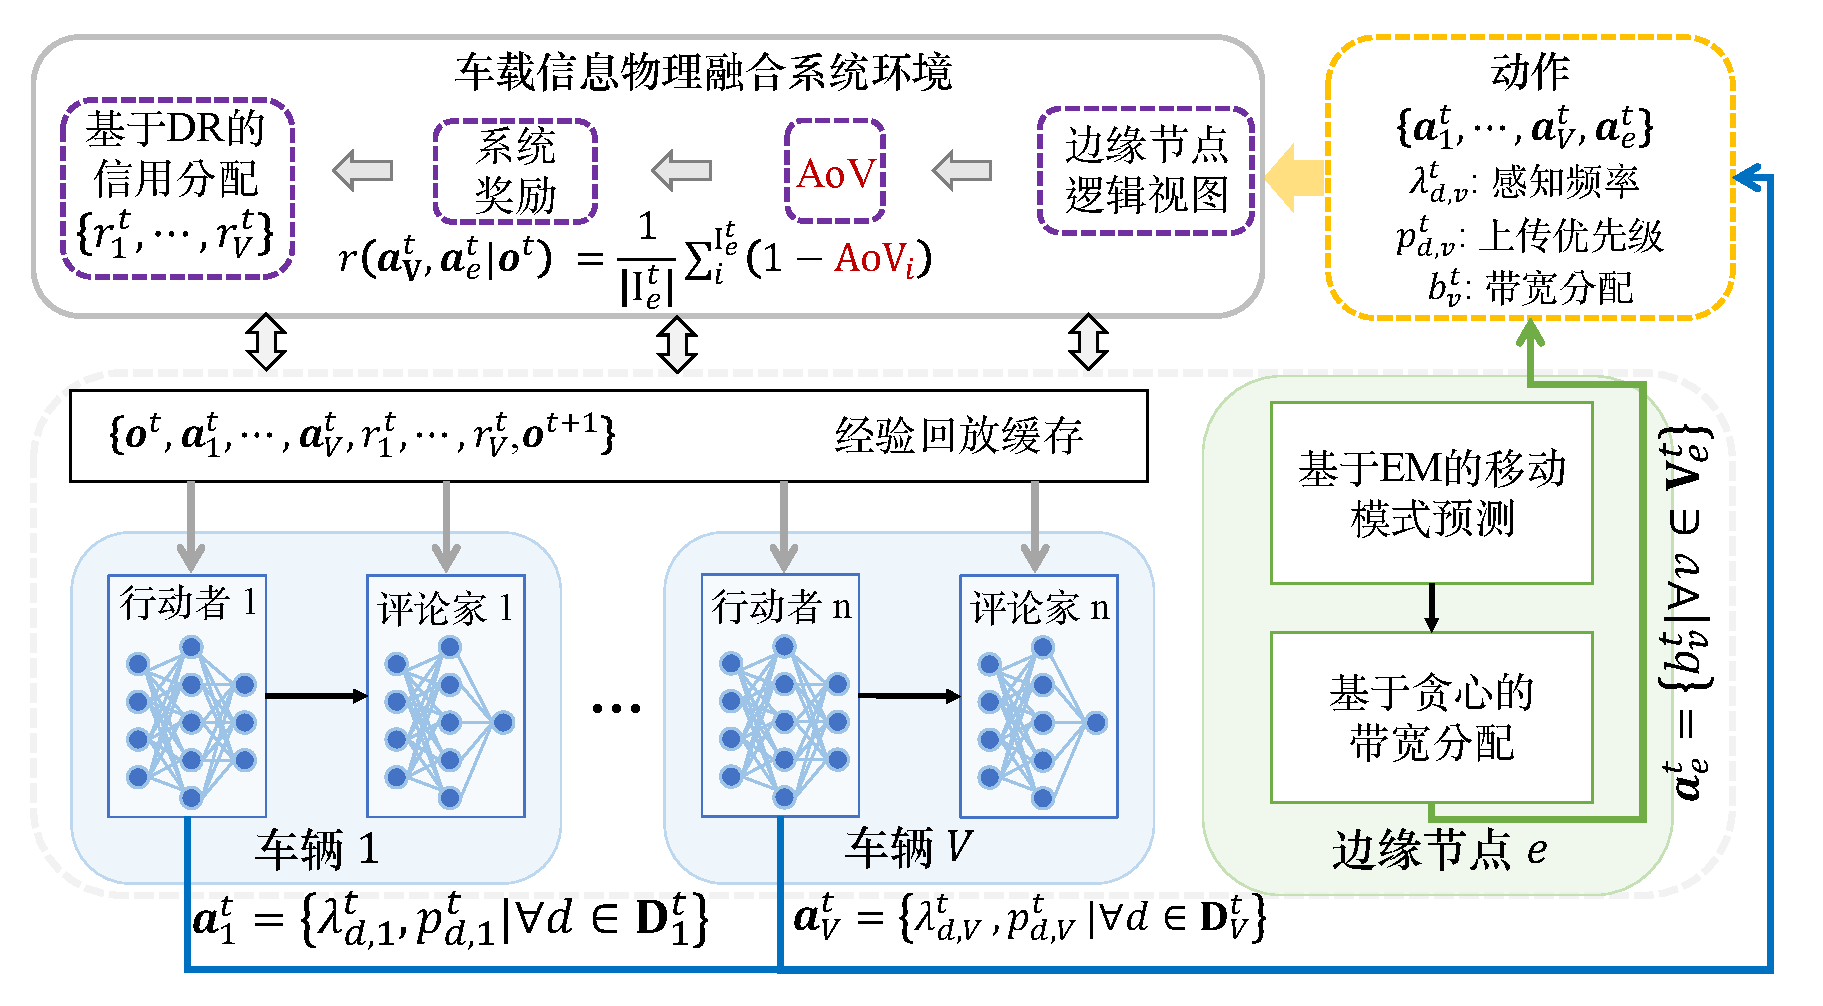
\includegraphics[width=0.6\textwidth]{fig/Fig2-4-solution-model.pdf}
\end{figure}
\end{textblock*}
\end{center}

\begin{center}
\begin{textblock*}{0.8\textwidth}(0cm,1.9cm)
\begin{itemize}[itemsep=0.2\baselineskip] \englishfont
	\item[\ding{111}] {\color{cqublue}{初始化}}
	\begin{itemize}[itemsep=0.2\baselineskip]
	\begin{small}
		\item[\ding{226}] 车辆行动者/评论家网络参数
		\item[\ding{226}] 经验回放缓存
		\end{small}
	\end{itemize}
	\item[\ding{111}]  {\color{cqublue}{回放经验存储}}
	\begin{itemize}[itemsep=0.2\baselineskip]
	\begin{small}
		\item[\ding{226}] 车辆决策{\small{$\boldsymbol{a}_{v}^{t}=\boldsymbol{\mu}_{\boldsymbol{v}}\left(\boldsymbol{o}_{v}^{t} \mid \theta_{v}^{\mu}\right)+\mathcal{N}_{t}$}}
		\item[\ding{226}] 边缘节点基于VBA机制分配带宽
		\item[\ding{226}] 存储与环境交互结果
	\end{small}
	\end{itemize}
	\item[\ding{111}]  {\color{cqublue}{训练}}
	\begin{itemize}[itemsep=0.2\baselineskip]
	\begin{small}
		\item[\ding{226}] 评论家网络损失函数\\{\small{$\mathcal{L}\left(\theta_{v}^{Q}\right)=\frac{1}{M} \Sigma_{m}\left(\eta_{m}-Q_{v}\left(\boldsymbol{o}_{v}^{m}, \boldsymbol{a}_{\mathbf{V}}^{m} \mid \theta_{v}^{Q}\right)\right)^{2}$}}
		\item[\ding{226}] 行动者网络策略梯度\\{\small{$\nabla_{\theta_{v}^{\mu}} \mathcal{J} \approx \frac{1}{M} \sum_{m} \nabla_{\boldsymbol{a}_{\mathbf{V}}^{m}} Q_{v}\left(\boldsymbol{o}_{v}^{m}, \boldsymbol{a}_{\mathbf{V}}^{m} \mid \theta_{v}^{Q}\right) \nabla_{\theta_{v}^{\mu}} \mu_{v}\left(\boldsymbol{o}_{v}^{m+1} \mid \theta_{v}^{\mu}\right)$}}
	\end{small}
	\end{itemize}
\end{itemize}
\end{textblock*}
\end{center}
\end{frame}

\begin{frame}
\frametitle{\englishfont \underline{算法}:MADR模型}
\newBackground
\begin{center}
\begin{textblock*}{\textwidth}(4.8cm,2.4cm)

\begin{figure}
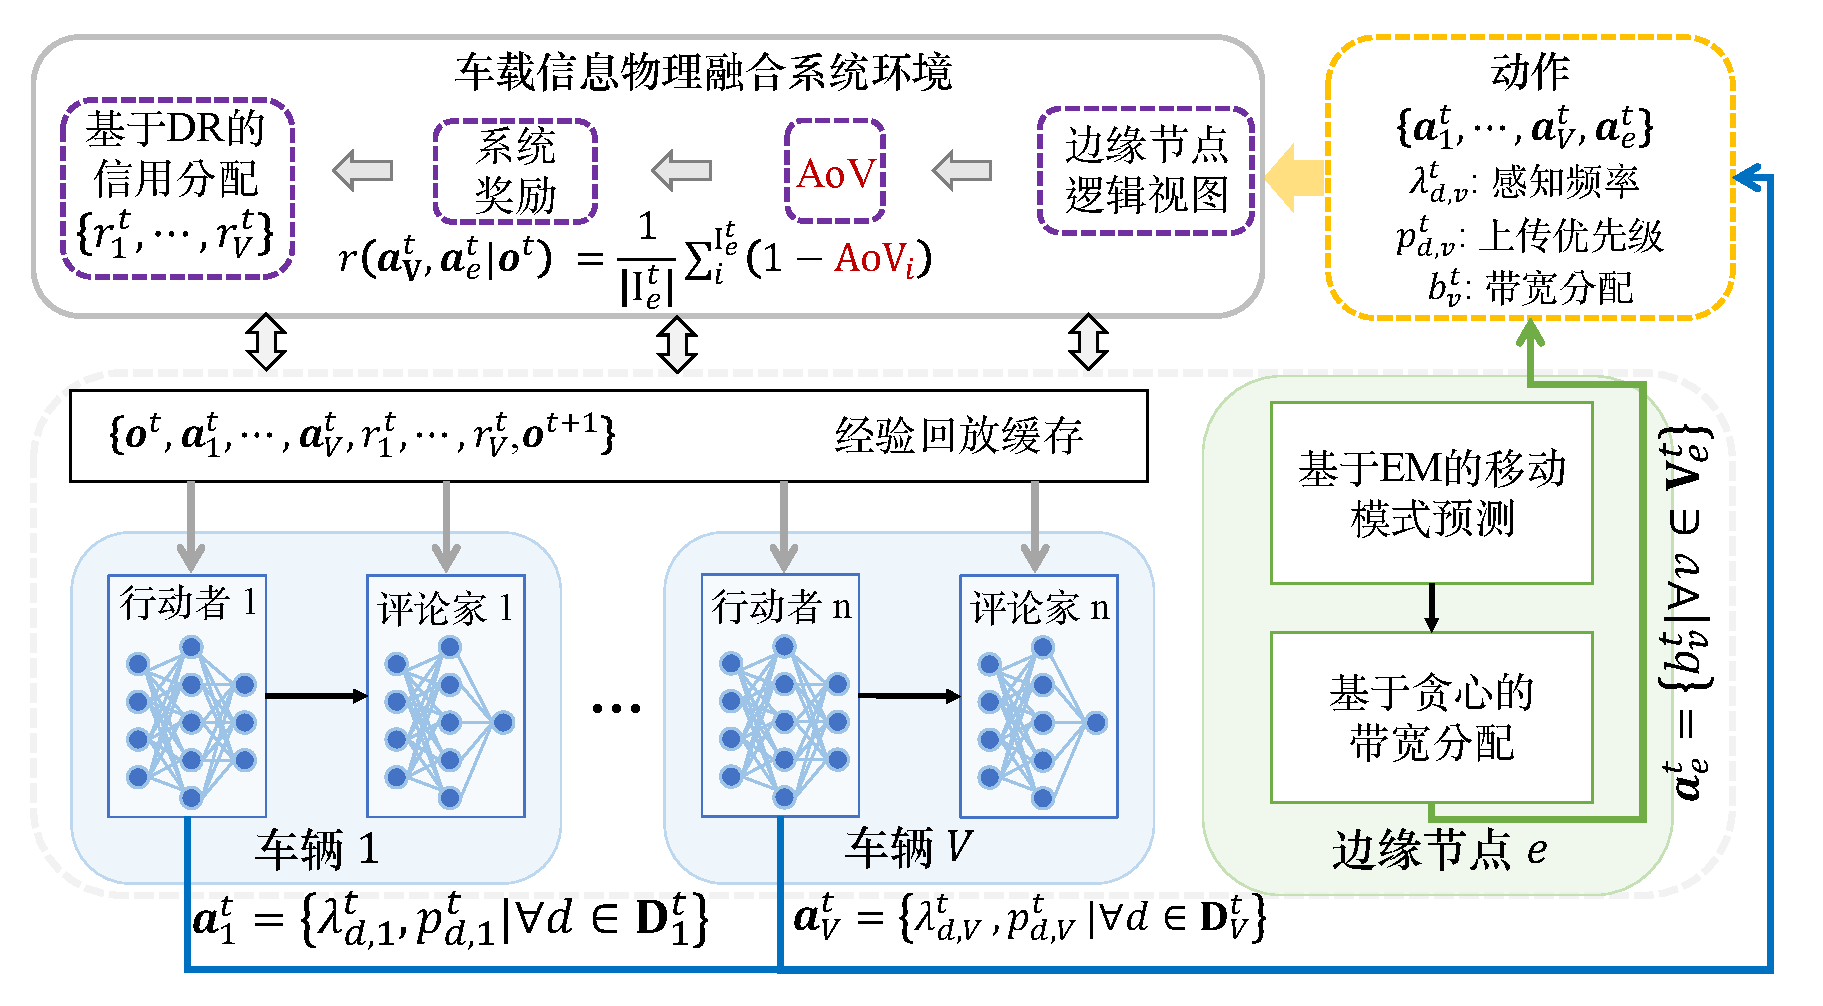
\includegraphics[width=0.6\textwidth]{fig/Fig2-4-solution-model.pdf}
\end{figure}
\end{textblock*}
\end{center}

\begin{center}
\begin{textblock*}{0.56\textwidth}(0.5cm,2cm)
\begin{itemize}[itemsep=0.2\baselineskip] \englishfont
	\item[\ding{111}] {\color{cqublue}{系统状态}}
	\begin{itemize}[itemsep=0.2\baselineskip]
	\begin{small}
		\item[\ding{226}] 车辆观测{\small{$\boldsymbol{o}_{v}^{t}=\left\{\mathbf{D}_{v}^{t}, \mathbf{D}_{e}^{t}, \mathbf{I}_e^t\right\}$}}
		\item[\ding{226}] {\small{$\boldsymbol{o}^{t}=\left\{\mathbf{D}_{1}^{t}, \ldots, \mathbf{D}_{v}^{t}, \ldots, \mathbf{D}_{V}^{t}, \mathbf{D}_{e}^{t}, \mathbf{I}_{e}^{t}\right\}$}}
	\end{small}
	\end{itemize}
	\item[\ding{111}]  {\color{cqublue}{动作空间}}
	\begin{itemize}[itemsep=0.2\baselineskip]
	\begin{small}
		\item[\ding{226}] {\small{$\boldsymbol{a}_{v}^{t}=\{ \lambda_{d, v}^{t}, p_{d, v}^{t} \mid \forall d \in \mathbf{D}_{v}^t\}$}}
		\item[\ding{226}] 车辆动作集合{\small{$\boldsymbol{a}_{\mathbf{V}}^{t} = \left\{\boldsymbol{a}_{v}^{t}\mid \forall v \in \mathbf{V}\right\}$}}
	\end{small}
	\end{itemize}
	\item[\ding{111}]  {\color{cqublue}{系统奖励}}
	\begin{itemize}[itemsep=0.2\baselineskip]
	\begin{small}
		\item[\ding{226}] {\small{$r\left(\boldsymbol{a}_{\mathbf{V}}^{t},\boldsymbol{a}_{e}^{t} \mid \boldsymbol{o}^{t}\right)=\frac{1}{\left|\mathbf{I}_e^t\right|} \sum_{\forall i \in \mathbf{I}_e^t}\left(1 -\operatorname{AoV}_{i} \right)$}}
		\item[\ding{226}] 车辆奖励:差分奖励分配机制\\{\small{$r_{v}^{t}=r\left(\boldsymbol{a}_{\mathbf{V}}^{t},\boldsymbol{a}_{e}^{t} \mid \boldsymbol{o}^{t}\right)-r\left(\boldsymbol{a}_{\mathbf{V}-v}^{t},\boldsymbol{a}_{e}^{t} \mid \boldsymbol{o}^{t}\right)$}}
	\end{small}
	\end{itemize}
\end{itemize}
\end{textblock*}
\end{center}
\end{frame}

\begin{frame}
\frametitle{\englishfont \underline{算法}:V2I 带宽分配机制 (VBA)}
\newBackground
\begin{center}
\begin{textblock*}{\textwidth}(4.8cm,2.4cm)
\begin{figure}
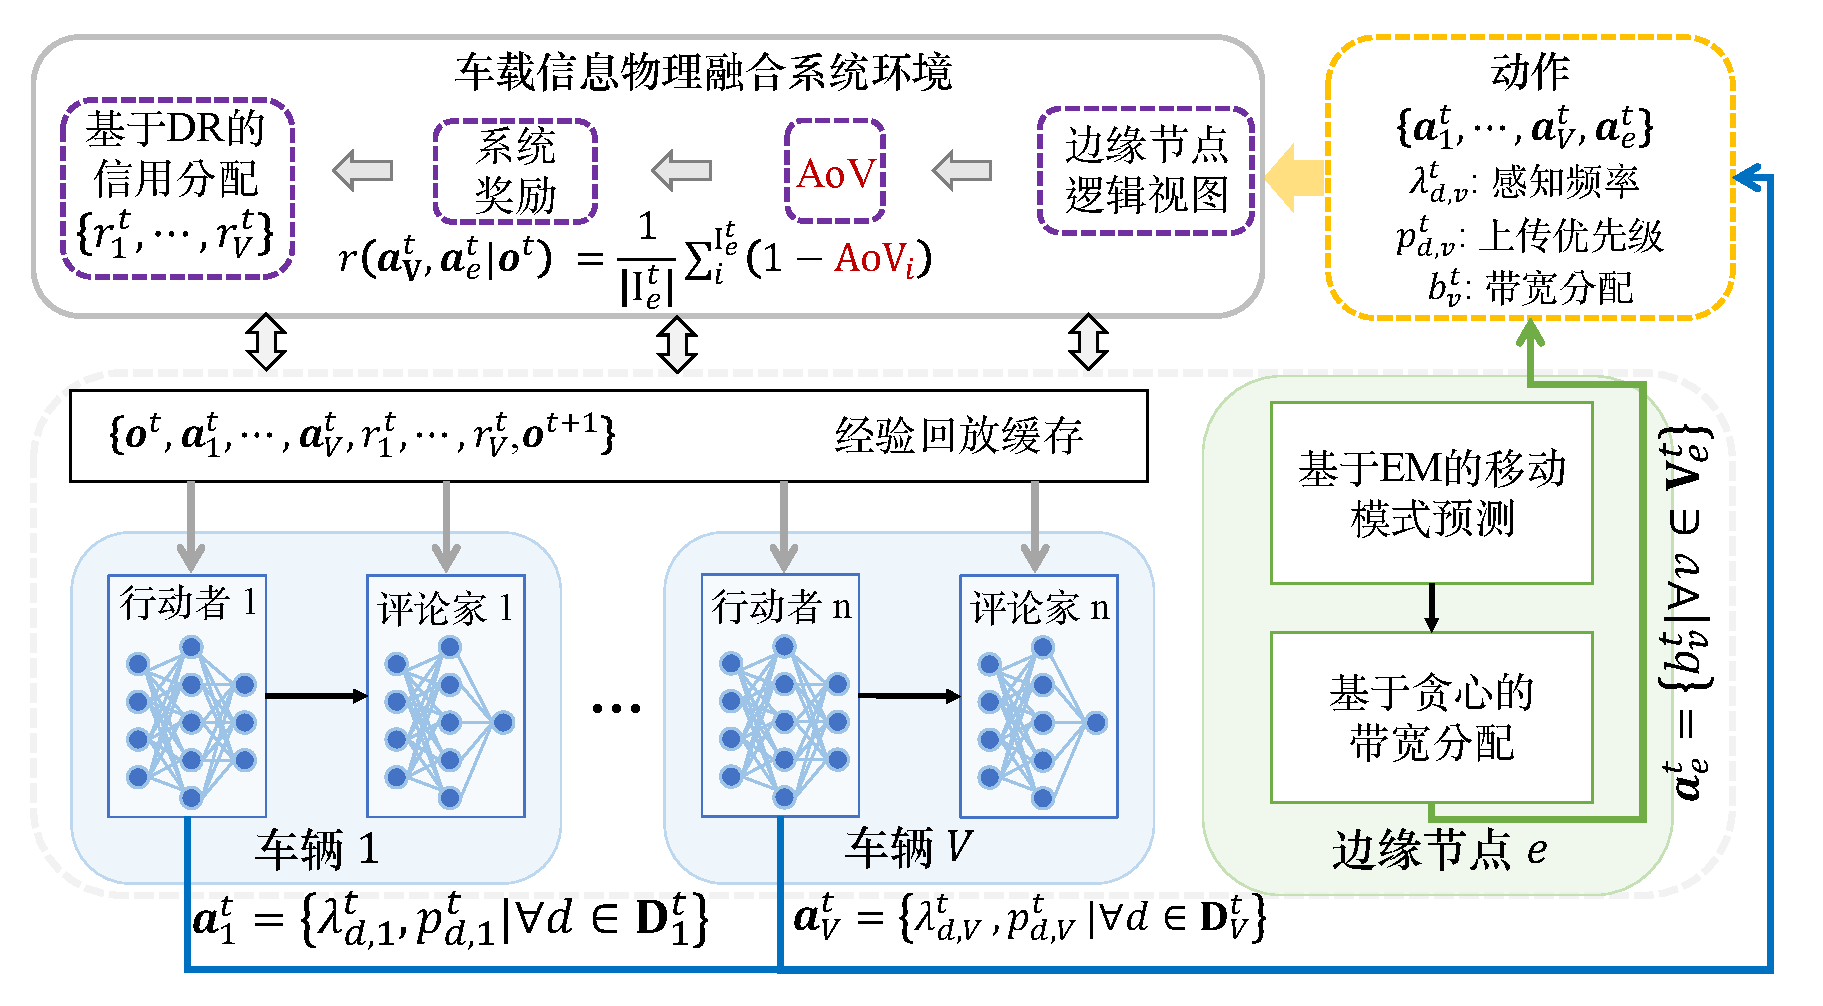
\includegraphics[width=0.6\textwidth]{fig/Fig2-4-solution-model.pdf}
\end{figure}
\end{textblock*}
\end{center}

\begin{center}
\begin{textblock*}{0.56\textwidth}(0.5cm,1.8cm)
\begin{itemize} \englishfont 
	\item[\ding{111}] {\color{cqublue}{距离估计}}
	\begin{itemize}[itemsep=0.2\baselineskip]
	\begin{small}
		\item[\ding{226}] 期望最大化 (EM)预测轨迹\\{\small{$\operatorname{Traj}_{v}^{t} = \{ \hat{l}_{v}^{t+1}, \dots, \hat{l}_{v}^{t+h}, \dots, \hat{l}_{v}^{t+H}\}$}}
		\item[\ding{226}] 平均距离{\small{$\operatorname{\bar{dis}}_{v, e}^{t} = \frac{1}{H} {\sum_{\forall h \in [1, H]} \widehat{\operatorname{dis}}_{v, e}^{t+h}}$}}
	\end{small}
	\end{itemize}
	\item[\ding{111}]  {\color{cqublue}{感知信息}}
	\begin{itemize}[itemsep=0.2\baselineskip]
	\begin{small}
		\item[\ding{226}] 视图$i$需要{\small{$\mathbf{D}_{v, i}^{t} = \left\{ d \mid  d \in \mathbf{D}_{v}^t \cap  \mathbf{D}_i \right\}$}}
		\item[\ding{226}] 视图需要{\small{$\mathbf{D}_{v, {\mathbf{I}_e^t}}^{t} = \{ d \mid  d \in \bigcup_{\forall v \in V_e^t} \mathbf{D}_{v, i}^{t}\}$}}
	\end{small}
	\end{itemize}
	\item[\ding{111}]  {\color{cqublue}{带宽分配}}
	\begin{itemize}[itemsep=0.2\baselineskip]
	\begin{small}
		\item[\ding{226}] {\small{$b_{v, e}^{t} =\frac{b_{e}} {\omega+\operatorname{rank}_{v}}$}}
		\item[\ding{226}] 按$| \mathbf{D}_{v, {\mathbf{I}_e^t}}^{t}|$的序列降序
		\item[\ding{226}] 按$\operatorname{\bar{dis}}_{v, e}^{t}$的序列升序
	\end{small}
	\end{itemize}
\end{itemize}
\end{textblock*}
\end{center}
\end{frame}


\begin{frame}
\frametitle{\englishfont \underline{实验}:数据与基本设置}
\newBackground

\begin{center}
	\begin{textblock*}{\textwidth}(-2.4cm,2.3cm)
	\begin{table}[h] \englishfont
\resizebox{0.45\textwidth}{!}{%
\begin{tabular}{cc}
\toprule 
\textbf{参数} & \textbf{值}         \\ \midrule
信息数据大小      & {[}100 B, 1 MB{]}  \\
传输功率        & 1 mW               \\
通信噪声        & -90 dBm            \\
带宽          & 3 MHz              \\
行动者         & 4 层全连接 (隐藏层 64-32)  \\
评论家         & 4 层全连接 (隐藏层 128-64) \\
学习率         & 0.001              \\
折扣因子        & 0.996              \\
经验回放缓存大小    & 100000             \\
批大小         & 512                \\ \bottomrule
\end{tabular}%
}
\end{table}
\end{textblock*}
\end{center}

\begin{center}
\begin{textblock*}{\textwidth}(0cm,1.8cm)
\begin{itemize} \englishfont \small
	\item[\ding{111}] {\color{cqublue}{实验与模型参数}}
\end{itemize}
\end{textblock*}
\end{center}

\begin{center}
\begin{textblock*}{\textwidth}(5cm,1.8cm)
	\begin{figure}
	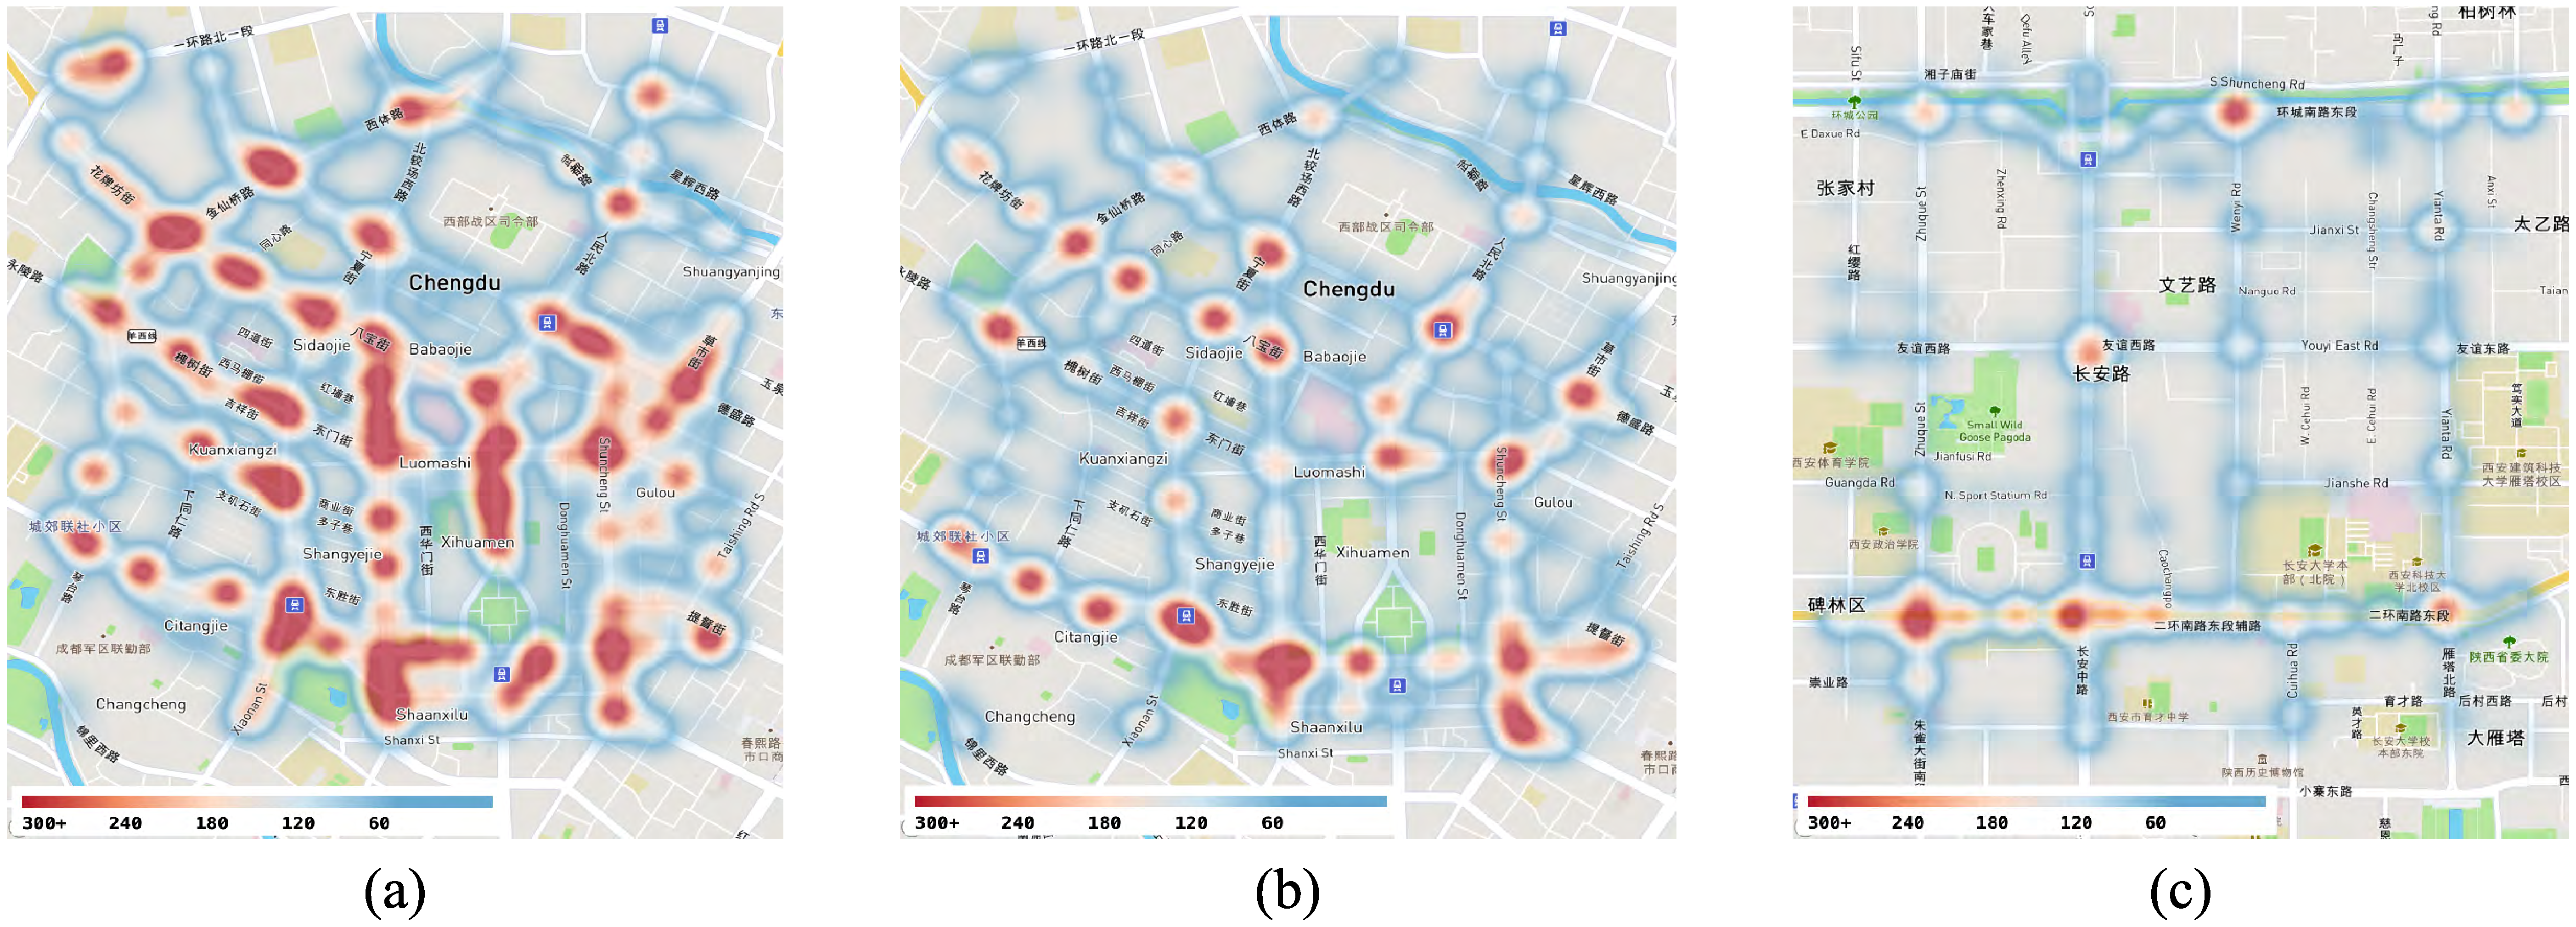
\includegraphics[width=0.5\textwidth]{fig/Fig2-5-heat-map.pdf}
	\end{figure}
\end{textblock*}
\end{center}

\begin{center}
\begin{textblock*}{\textwidth}(0cm,6.5cm)
\begin{itemize} \englishfont 
	\item[\ding{111}] {\color{cqublue}{对比算法}}
	\begin{itemize}
	\begin{small}
		\item[\ding{226}] 随机分配 ({\color{red}{RA}})、深度确定性策略梯度 ({\color{red}{DDPG}})
		\item[\ding{226}] 多智能体行动者-评论家 ({\color{red}{MAAC}})
		\item[\ding{226}] 采用VBA策略的MAAC ({\color{red}{MAAC-VBA}})
		\item
	\end{small}
	\end{itemize}
\end{itemize}
\end{textblock*}
\end{center}

\begin{center}
\begin{textblock*}{0.55\textwidth}(8.2cm,4.5cm)
\begin{itemize}[itemsep=0.2\baselineskip] \englishfont
	\item[\ding{111}] {\color{cqublue}{性能评估指标}}
	\begin{itemize}[itemsep=0.2\baselineskip]
	\begin{small}
		\item[\ding{226}] 累计奖励 ({\color{red}{CR}})
		\item[\ding{226}] 平均奖励的构成 ({\color{red}{CAR}})\\{\small{$<\frac{3}{10}(1-\hat{\Xi}_{i}),\frac{4}{10}(1-\hat{\Phi}_{i}), \frac{3}{10}(1-\hat{\Psi}_{i})>$}}
		\item[\ding{226}] 平均排队时间 ({\color{red}{AQT}})
		\item[\ding{226}] 服务率 ({\color{red}{SR}})
	\end{small}
	\end{itemize}
\end{itemize}
\end{textblock*}
\end{center}

\end{frame}

\begin{frame}
\newBackground

\begin{overlayarea}{\textwidth}{3cm}
\only<1-1>{
\frametitle{\englishfont \underline{实验}:算法收敛性}
\begin{center} \englishfont \footnotesize
\begin{textblock*}{\textwidth}(1cm,1.8cm)
	\begin{figure}
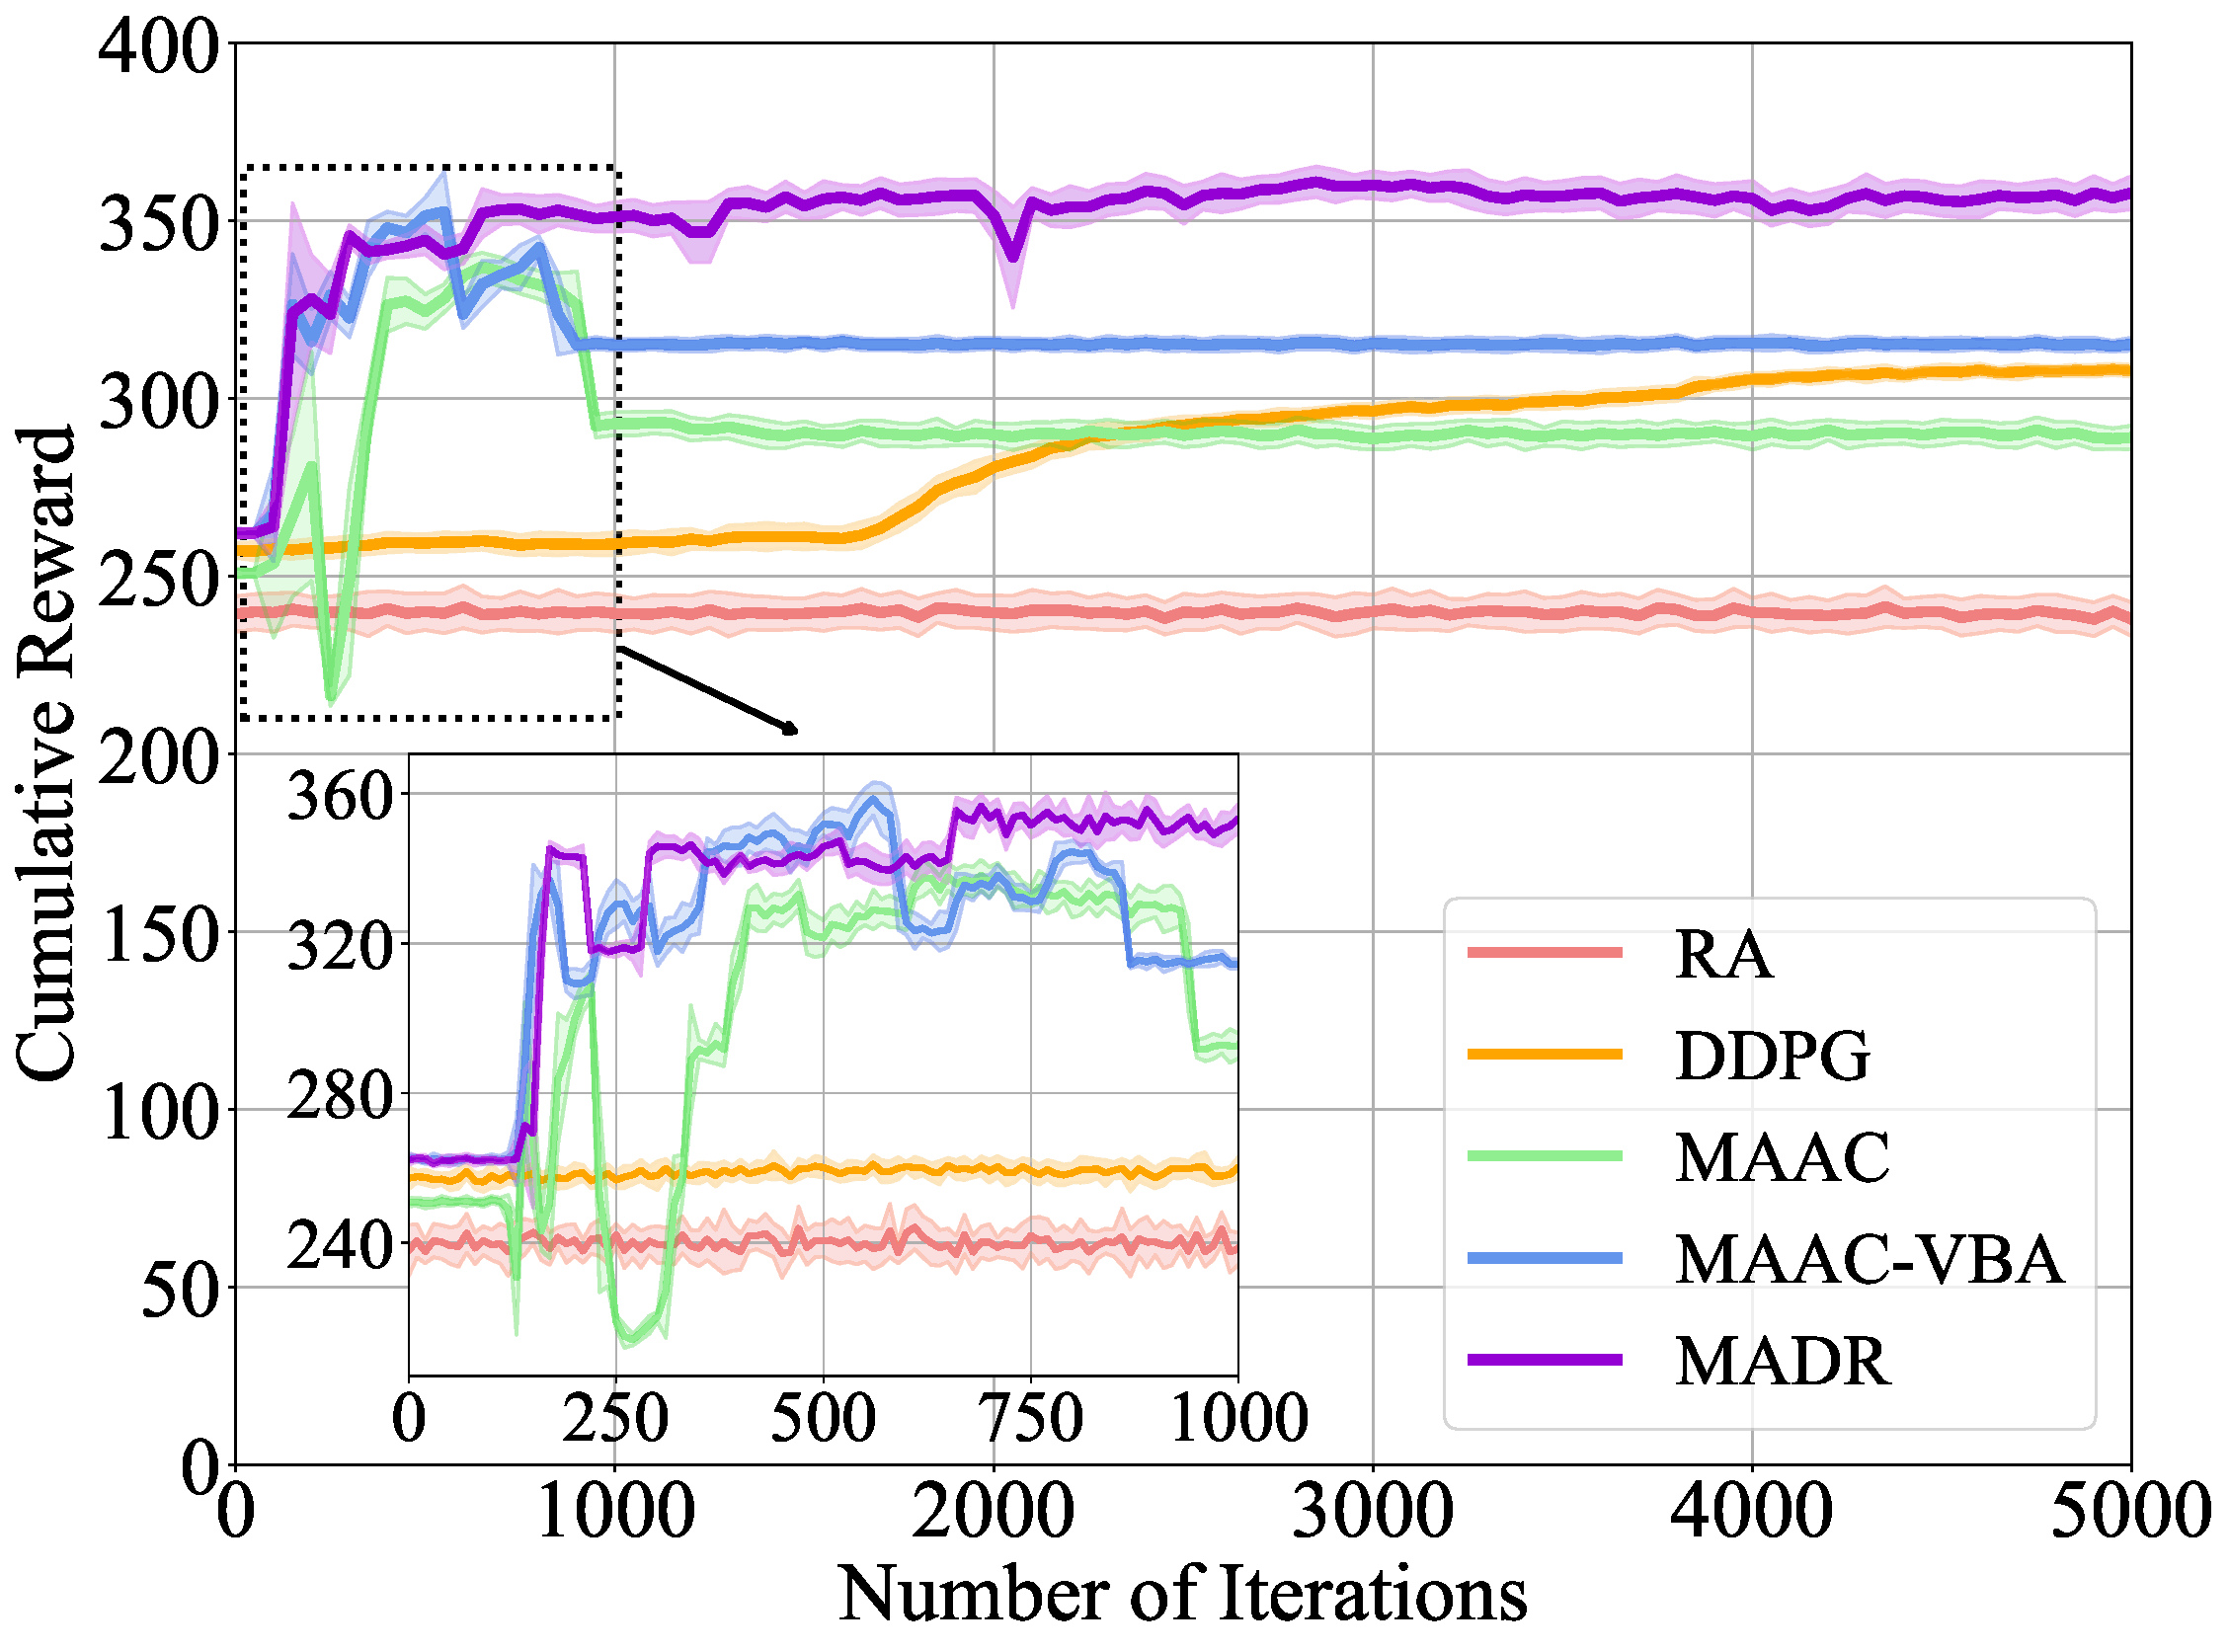
\includegraphics[width=0.6\textwidth]{fig/Fig2-6-convergence.pdf}
	\end{figure}
\end{textblock*}
\end{center}
}

\only<2-2>{
\frametitle{\englishfont \underline{实验}:算法收敛性}
\begin{center} \englishfont \footnotesize
\begin{textblock*}{\textwidth}(1cm,1.8cm)
	\begin{figure}
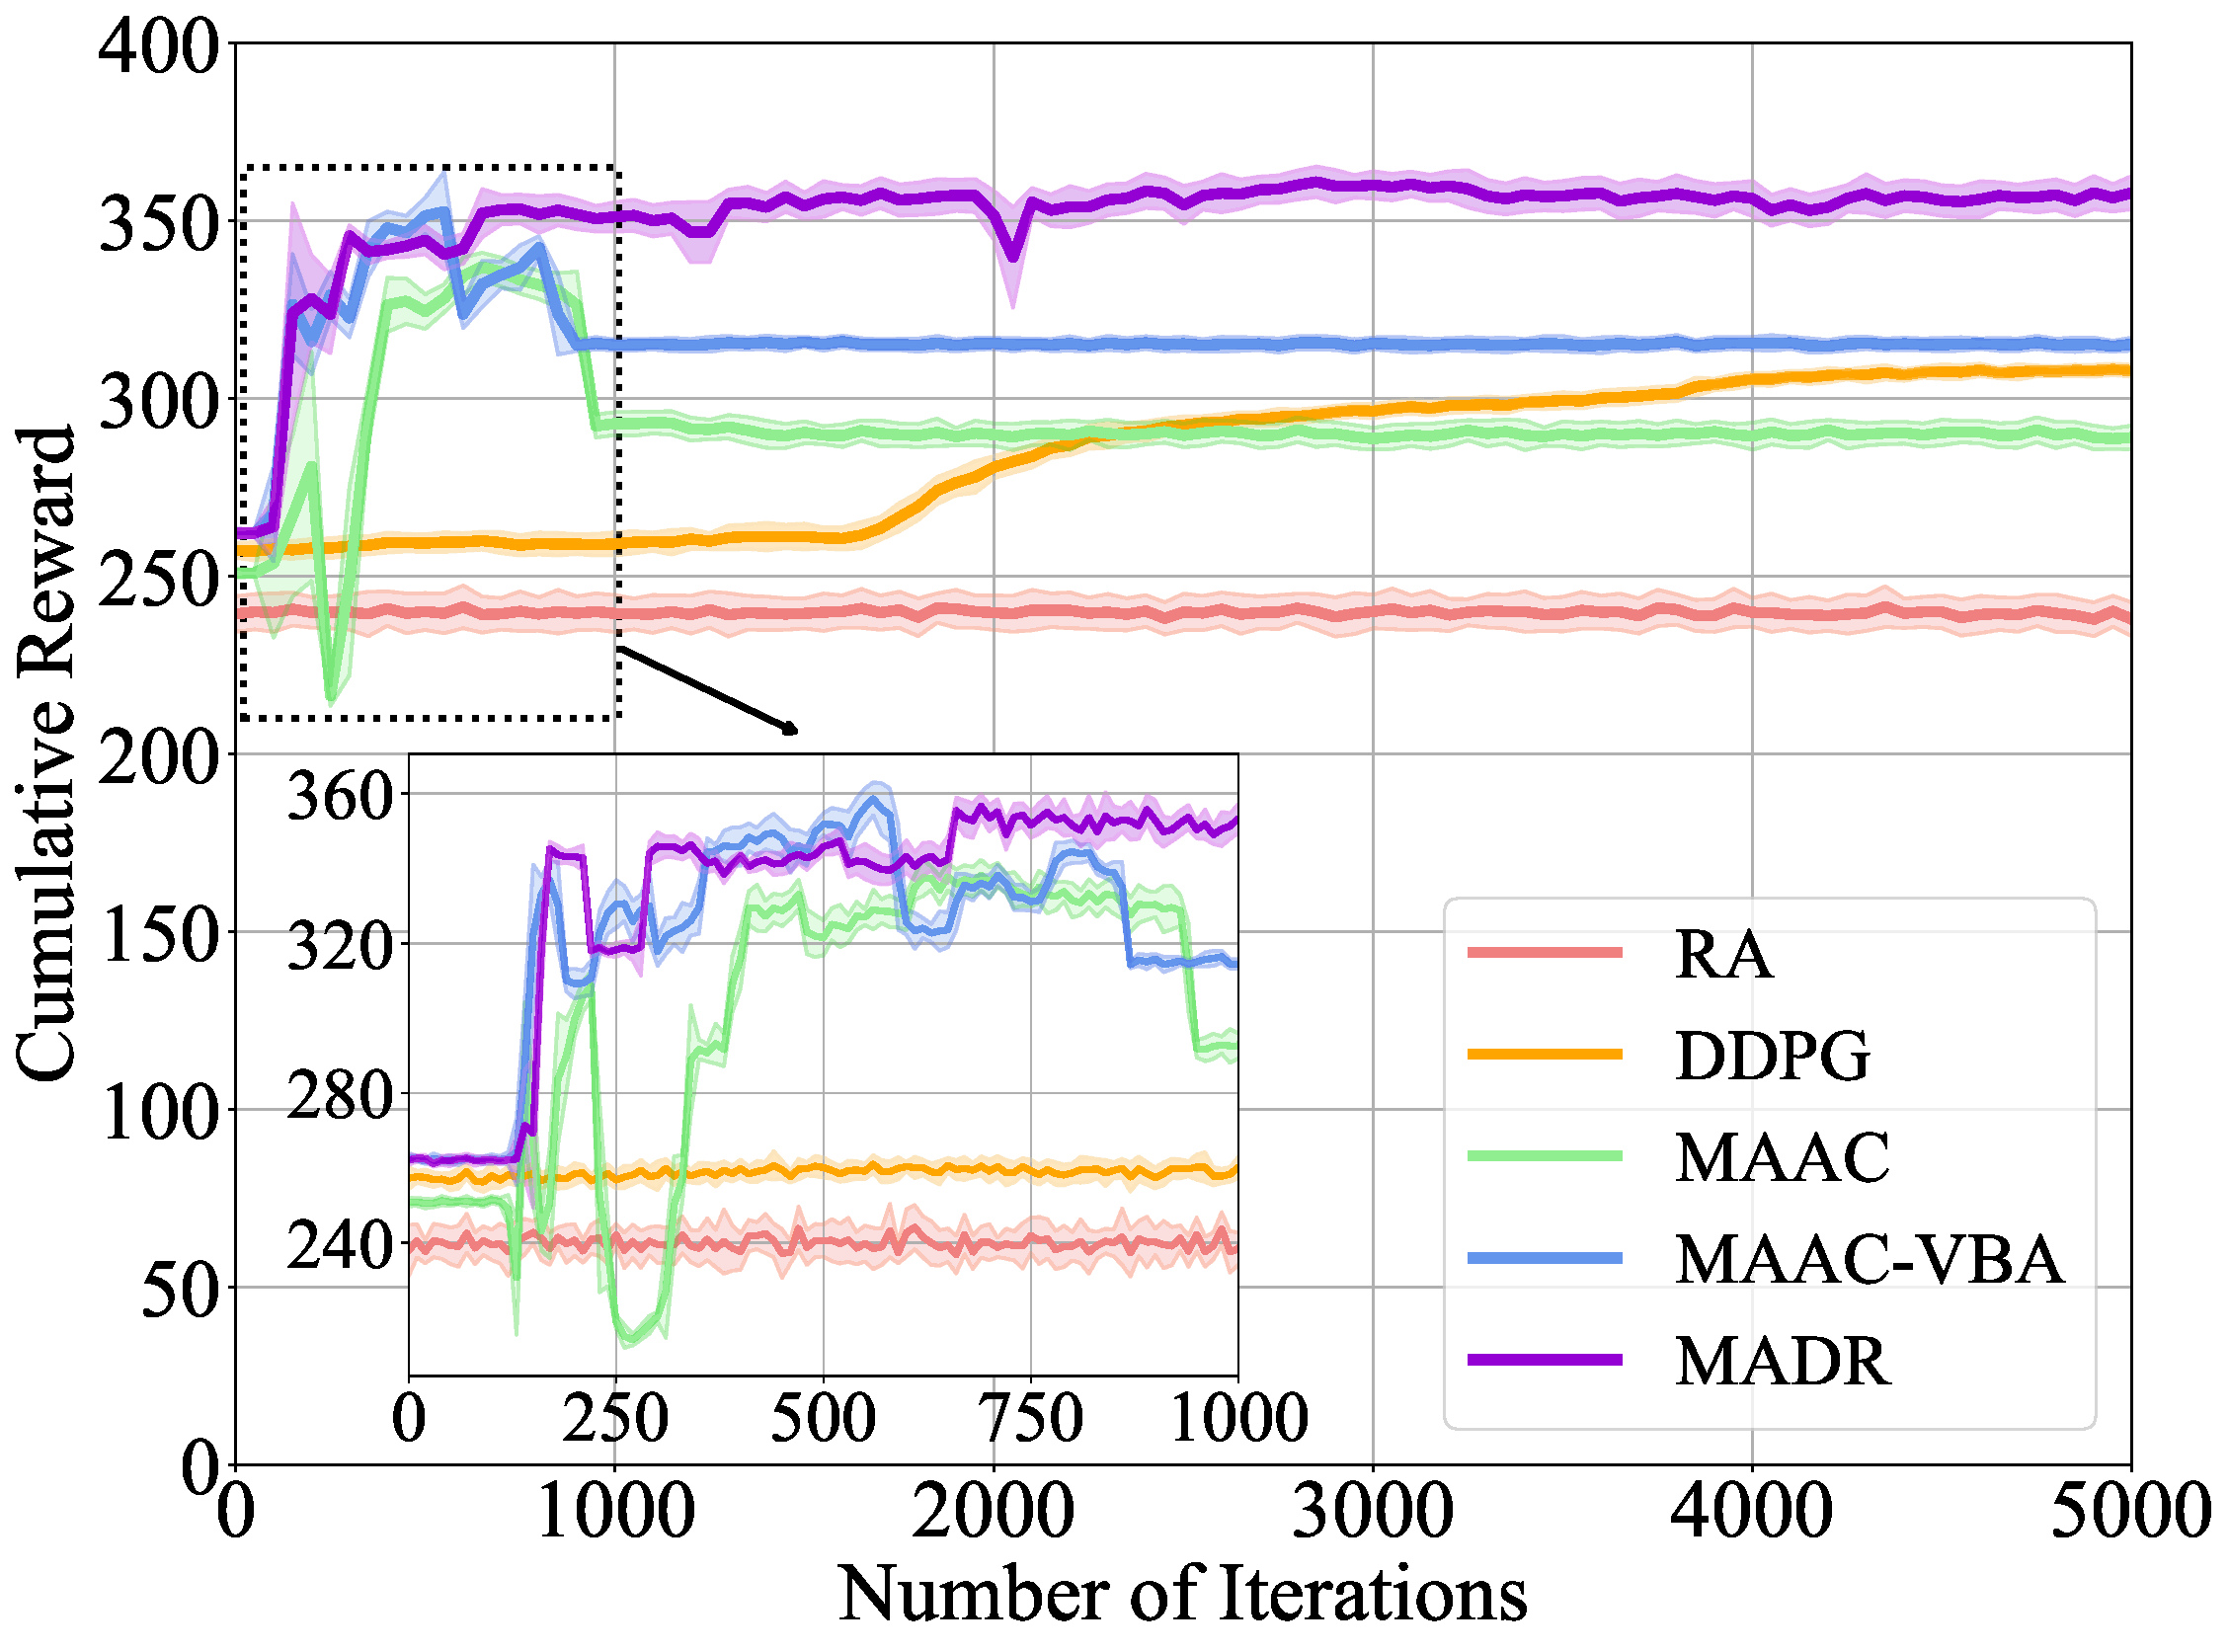
\includegraphics[width=0.6\textwidth]{fig/Fig2-6-convergence.pdf}
	\end{figure}
\end{textblock*}
\end{center}
}

\only<2-2>{
\begin{center} \englishfont \footnotesize
\begin{textblock*}{\textwidth}(1cm,1.9cm)
{\Huge{\color{red}\ding{216}}}
\end{textblock*}
\end{center}
}

\only<3-3>{
\frametitle{\englishfont \underline{实验}:交通场景的影响}
\begin{center} \englishfont \footnotesize
\begin{textblock*}{\textwidth}(1cm,1.8cm)
	\begin{figure}
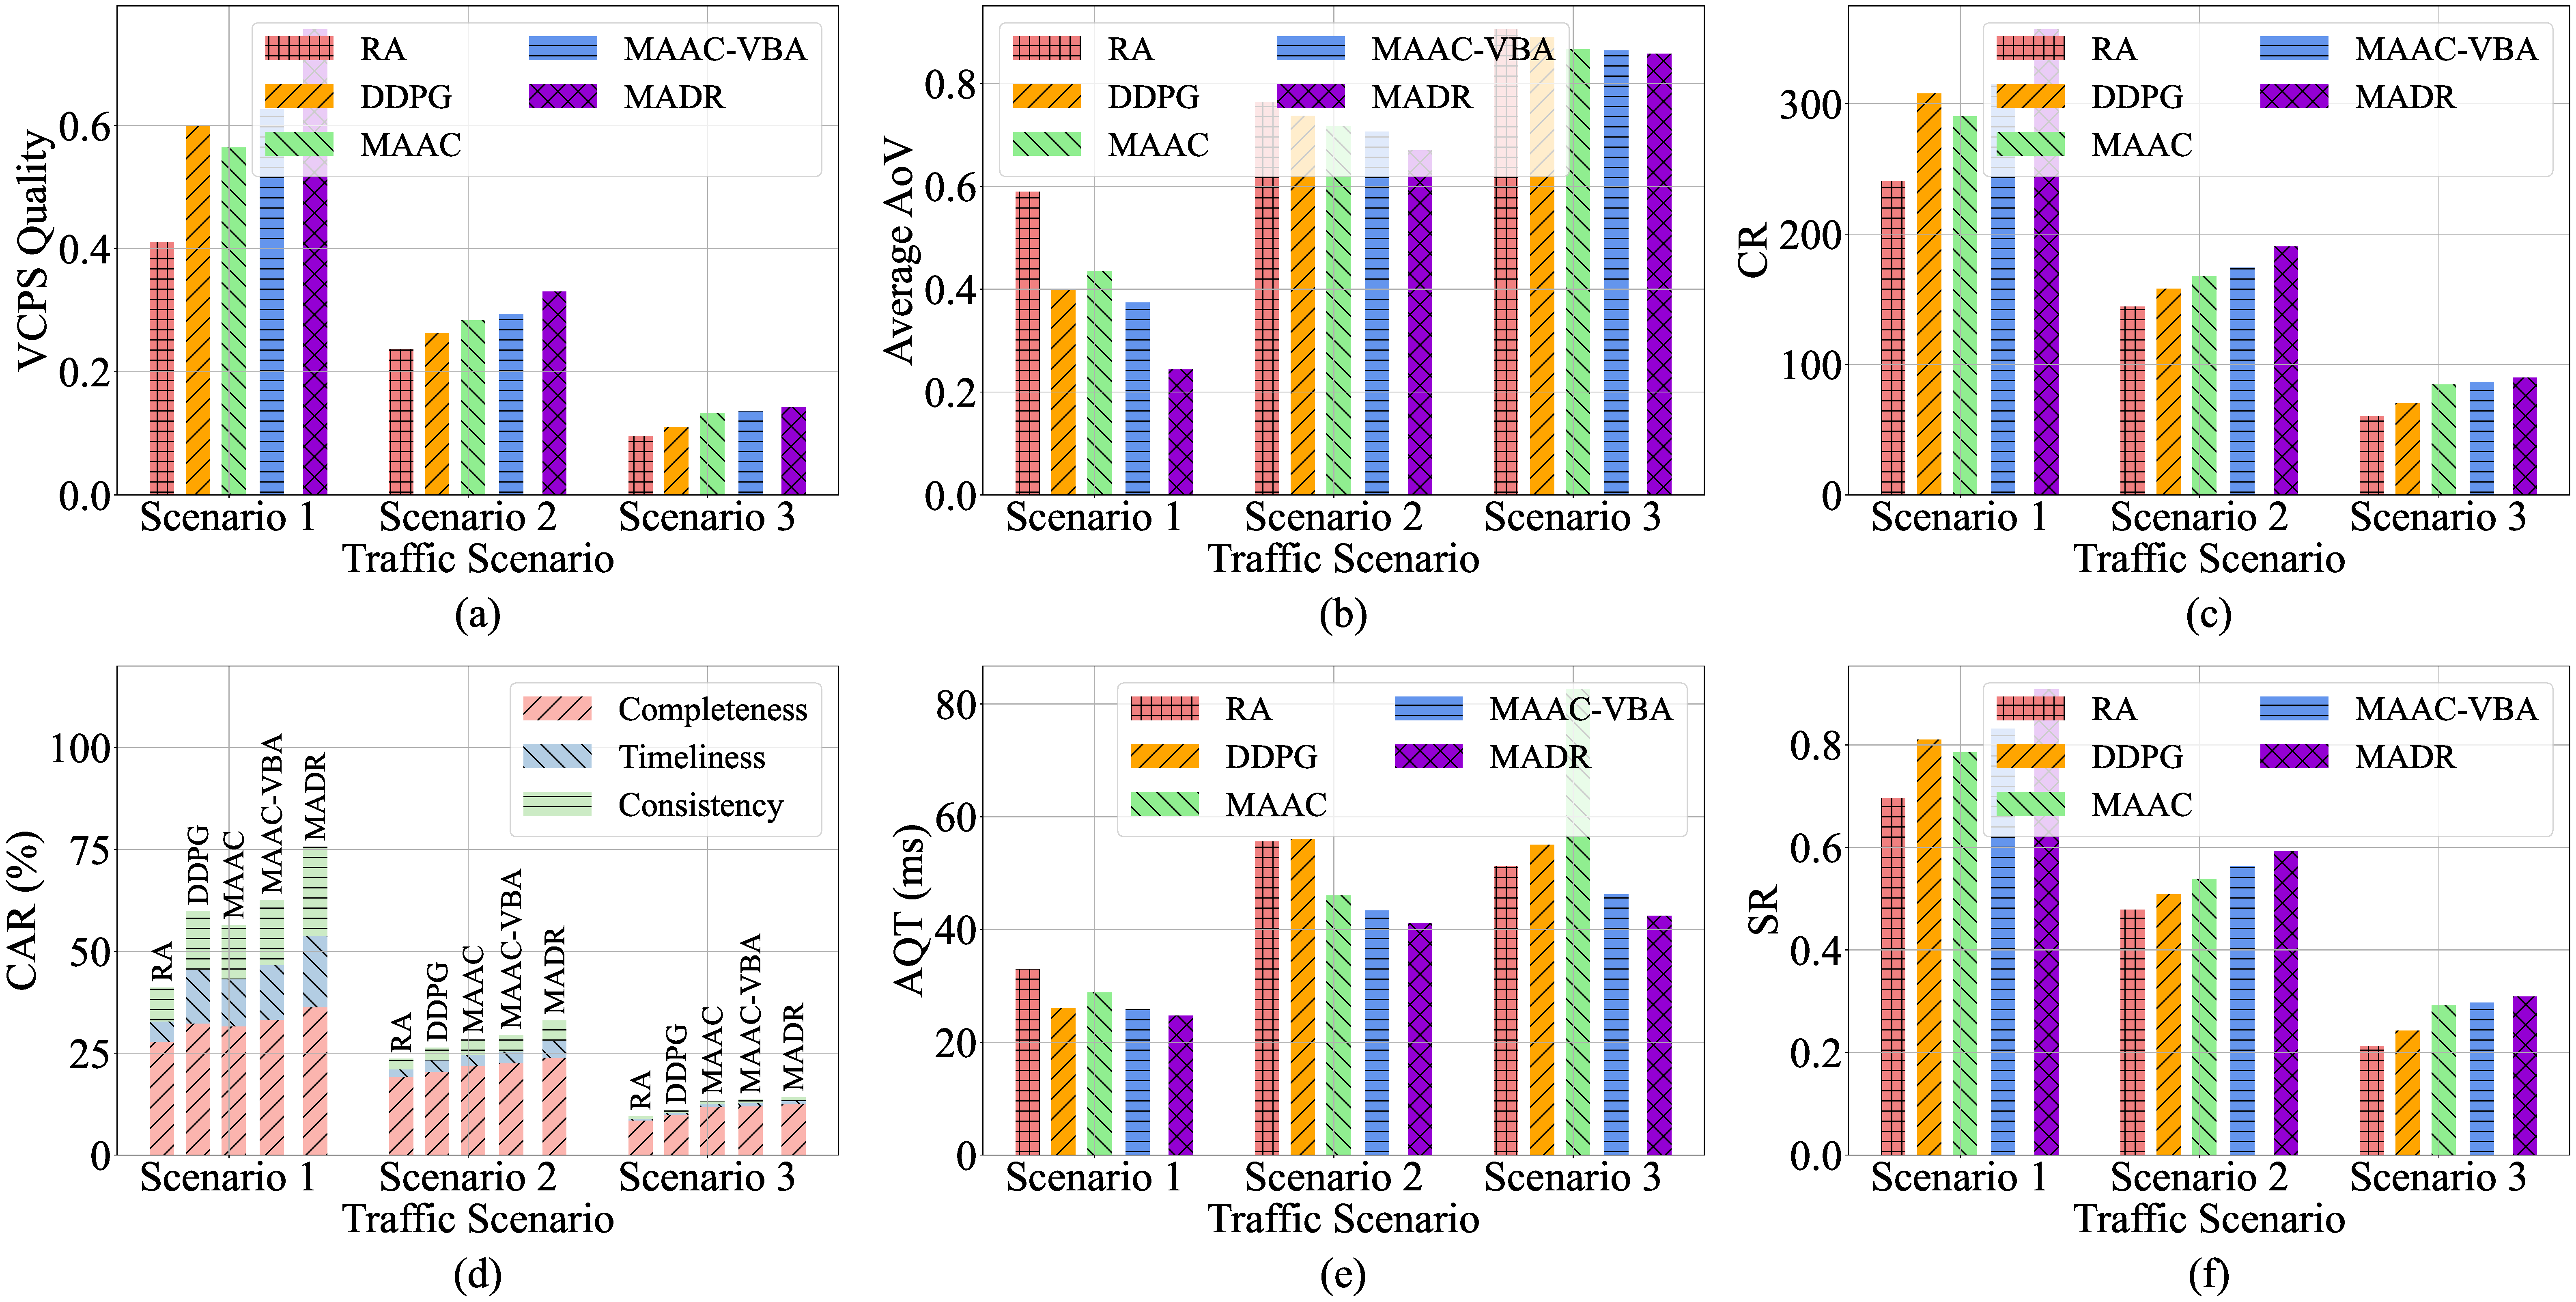
\includegraphics[width=0.9\textwidth]{fig/Fig2-7-different-scenarios.pdf}
	\end{figure}
\end{textblock*}
\end{center}
}

\only<4-4>{
\frametitle{\englishfont \underline{实验}:交通场景的影响}
\begin{center} \englishfont \footnotesize
\begin{textblock*}{\textwidth}(1cm,1.8cm)
	\begin{figure}
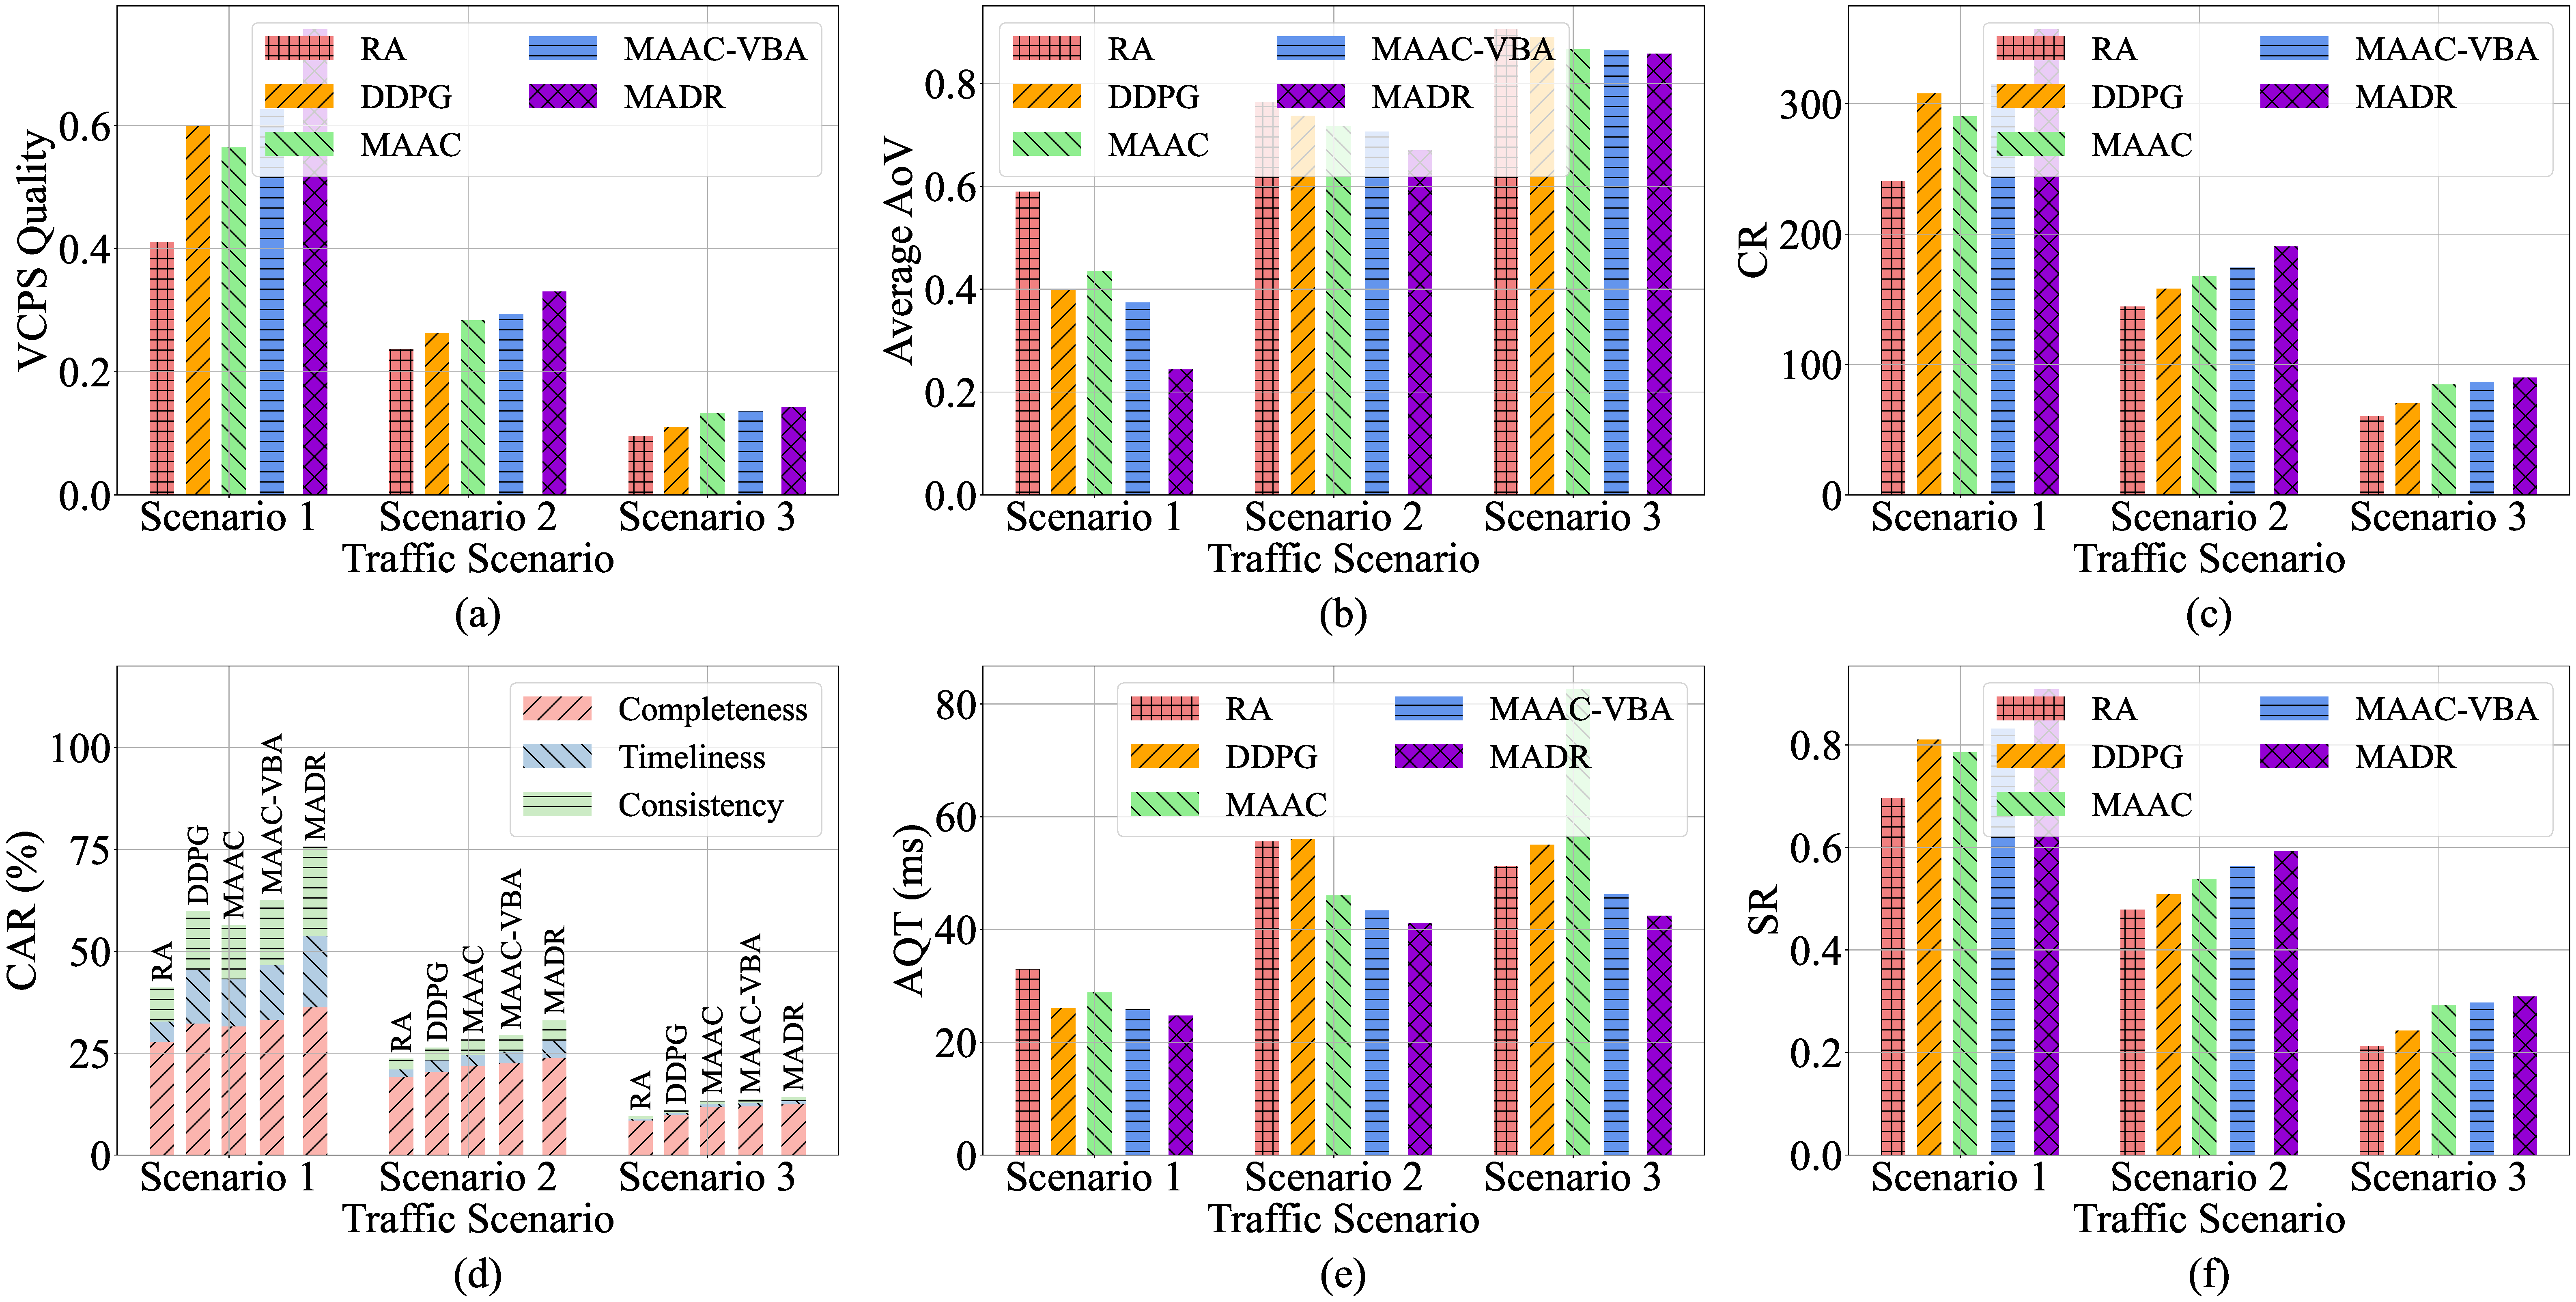
\includegraphics[width=0.9\textwidth]{fig/Fig2-7-different-scenarios.pdf}
	\end{figure}
\end{textblock*}
\end{center}
}

\only<4-4>{
\begin{center} \englishfont \footnotesize
\begin{textblock*}{\textwidth}(-1.6cm,3.4cm)
{\LARGE{\color{red}\ding{216}}}
\end{textblock*}
\end{center}

\begin{center} \englishfont \footnotesize
\begin{textblock*}{\textwidth}(0.3cm,3.25cm)
{\LARGE{\color{red}\ding{216}}}
\end{textblock*}
\end{center}

\begin{center} \englishfont \footnotesize
\begin{textblock*}{\textwidth}(5.7cm,2.65cm)
{\LARGE{\color{red}\ding{216}}}
\end{textblock*}
\end{center}

\begin{center} \englishfont \footnotesize
\begin{textblock*}{\textwidth}(2.6cm,5.9cm)
{\LARGE{\color{red}\ding{216}}}
\end{textblock*}
\end{center}

\begin{center} \englishfont \footnotesize
\begin{textblock*}{\textwidth}(6.85cm,6.3cm)
{\LARGE{\color{red}\ding{216}}}
\end{textblock*}
\end{center}
}

\only<5-5>{
\frametitle{\englishfont \underline{实验}:V2I带宽的影响}
\begin{center} \englishfont \footnotesize
\begin{textblock*}{\textwidth}(1cm,1.8cm)
	\begin{figure}
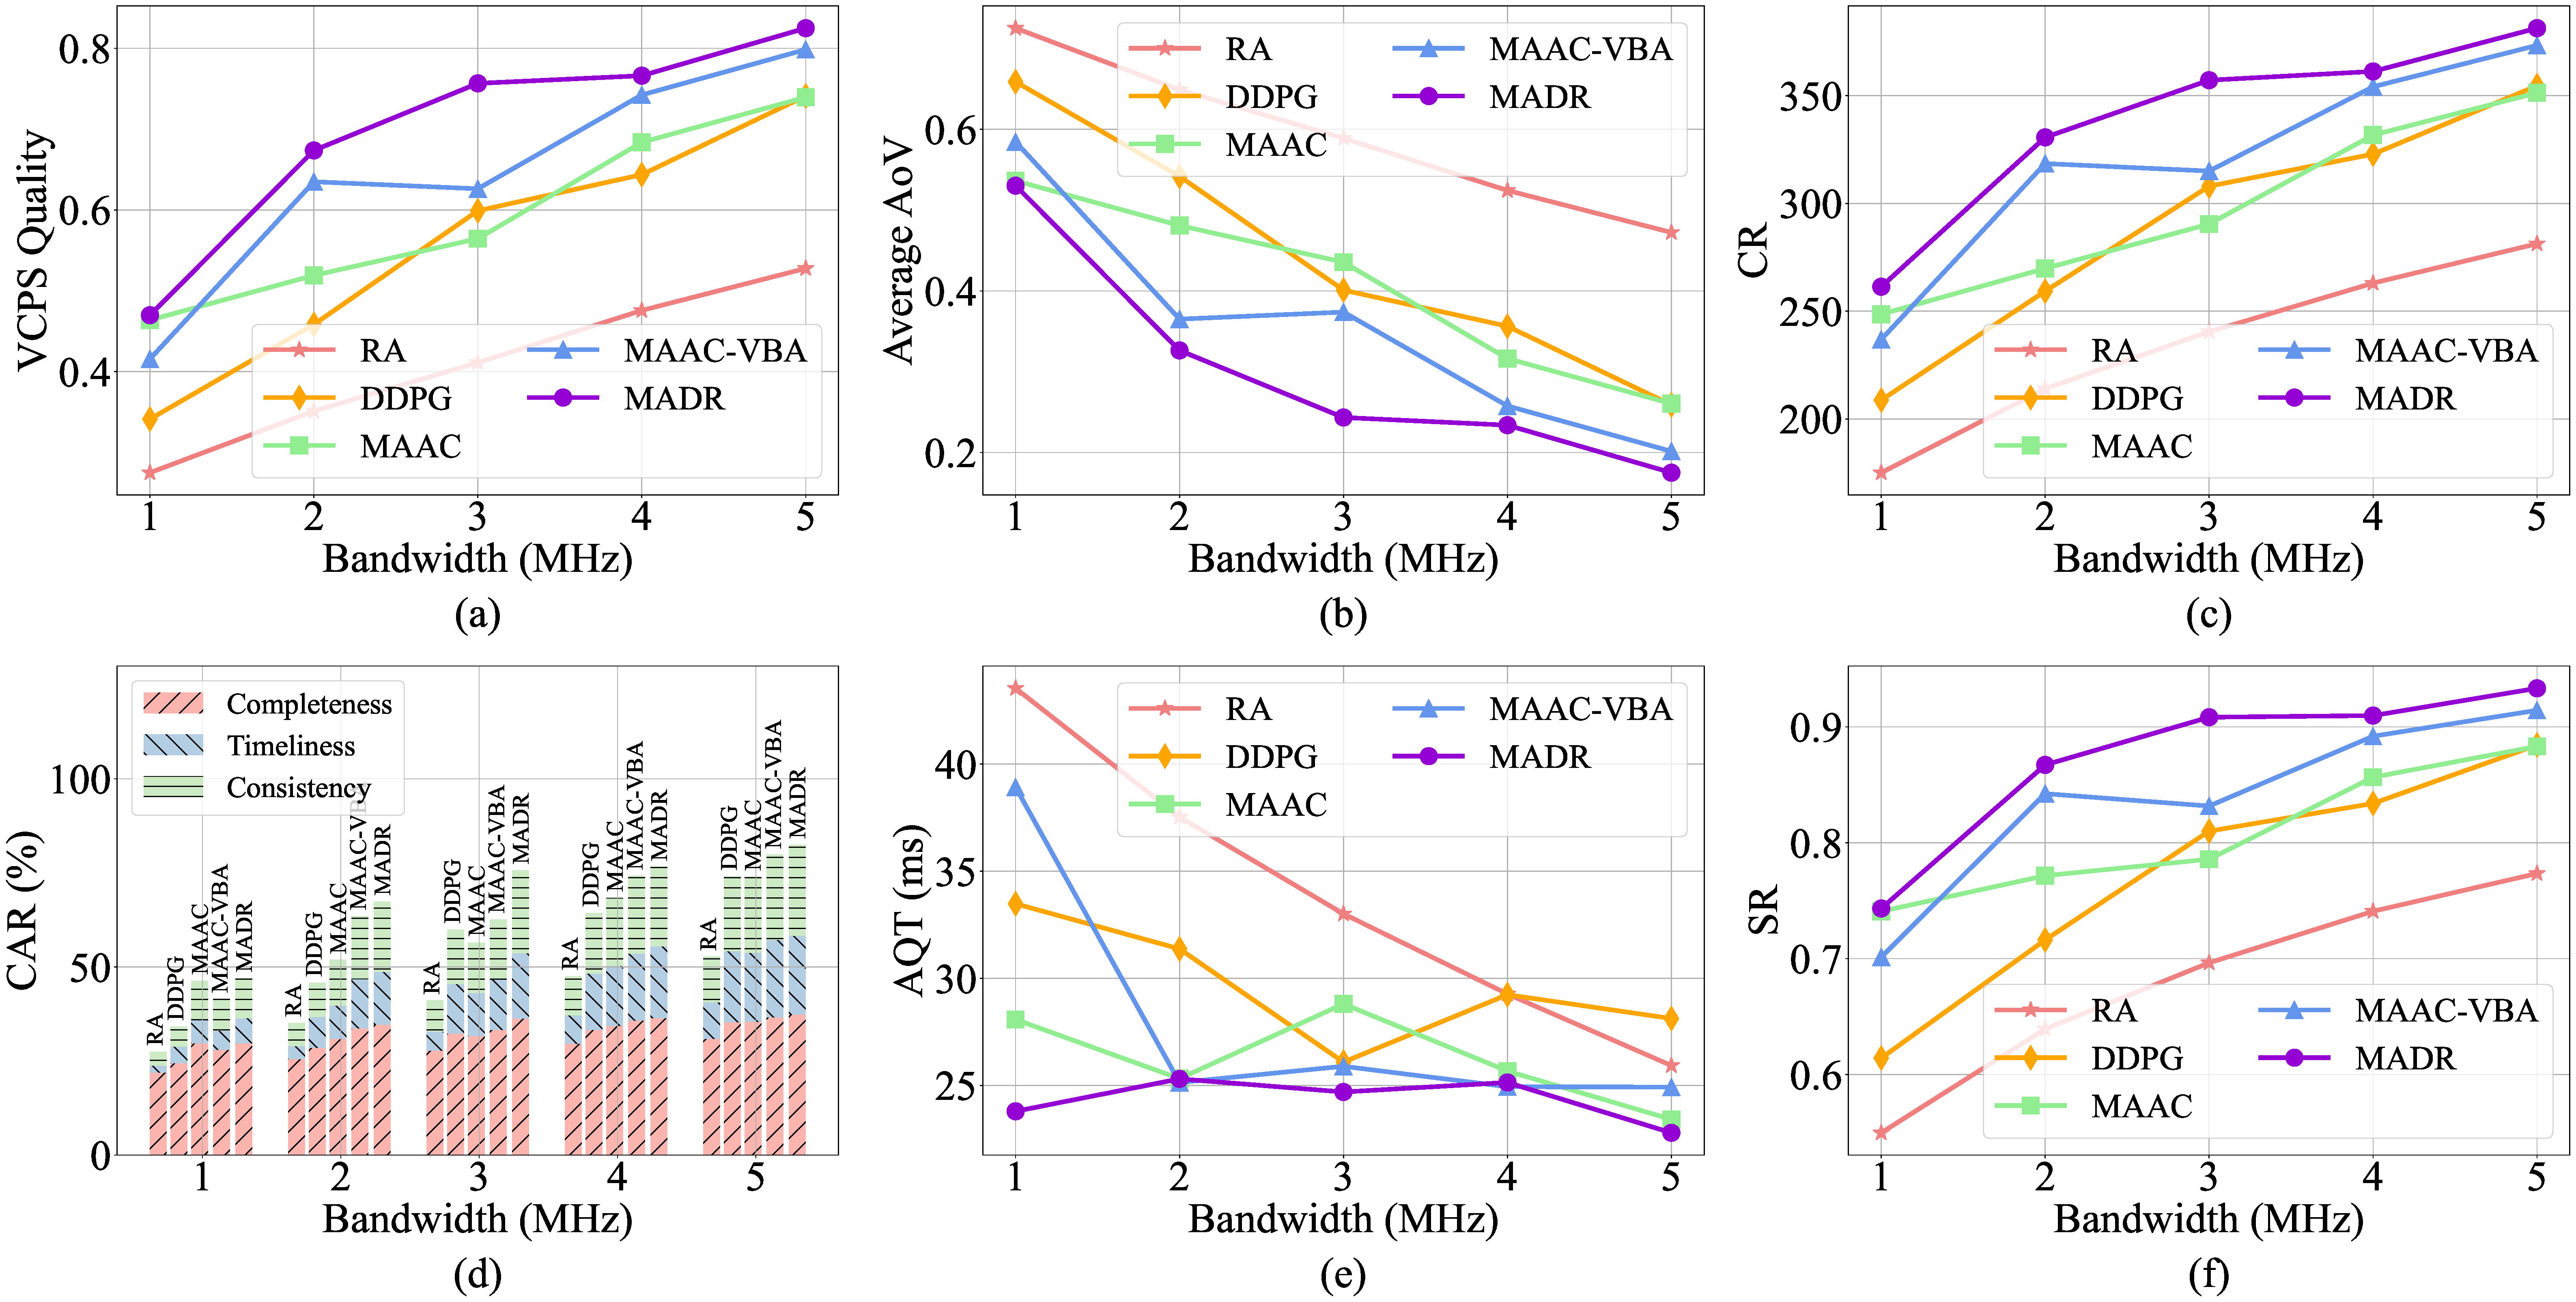
\includegraphics[width=0.9\textwidth]{fig/Fig2-8-different-bandwidths.pdf}
	\end{figure}
\end{textblock*}
\end{center}
}

\only<6-6>{
\frametitle{\englishfont \underline{实验}:V2I带宽的影响}
\begin{center} \englishfont \footnotesize
\begin{textblock*}{\textwidth}(1cm,1.8cm)
	\begin{figure}
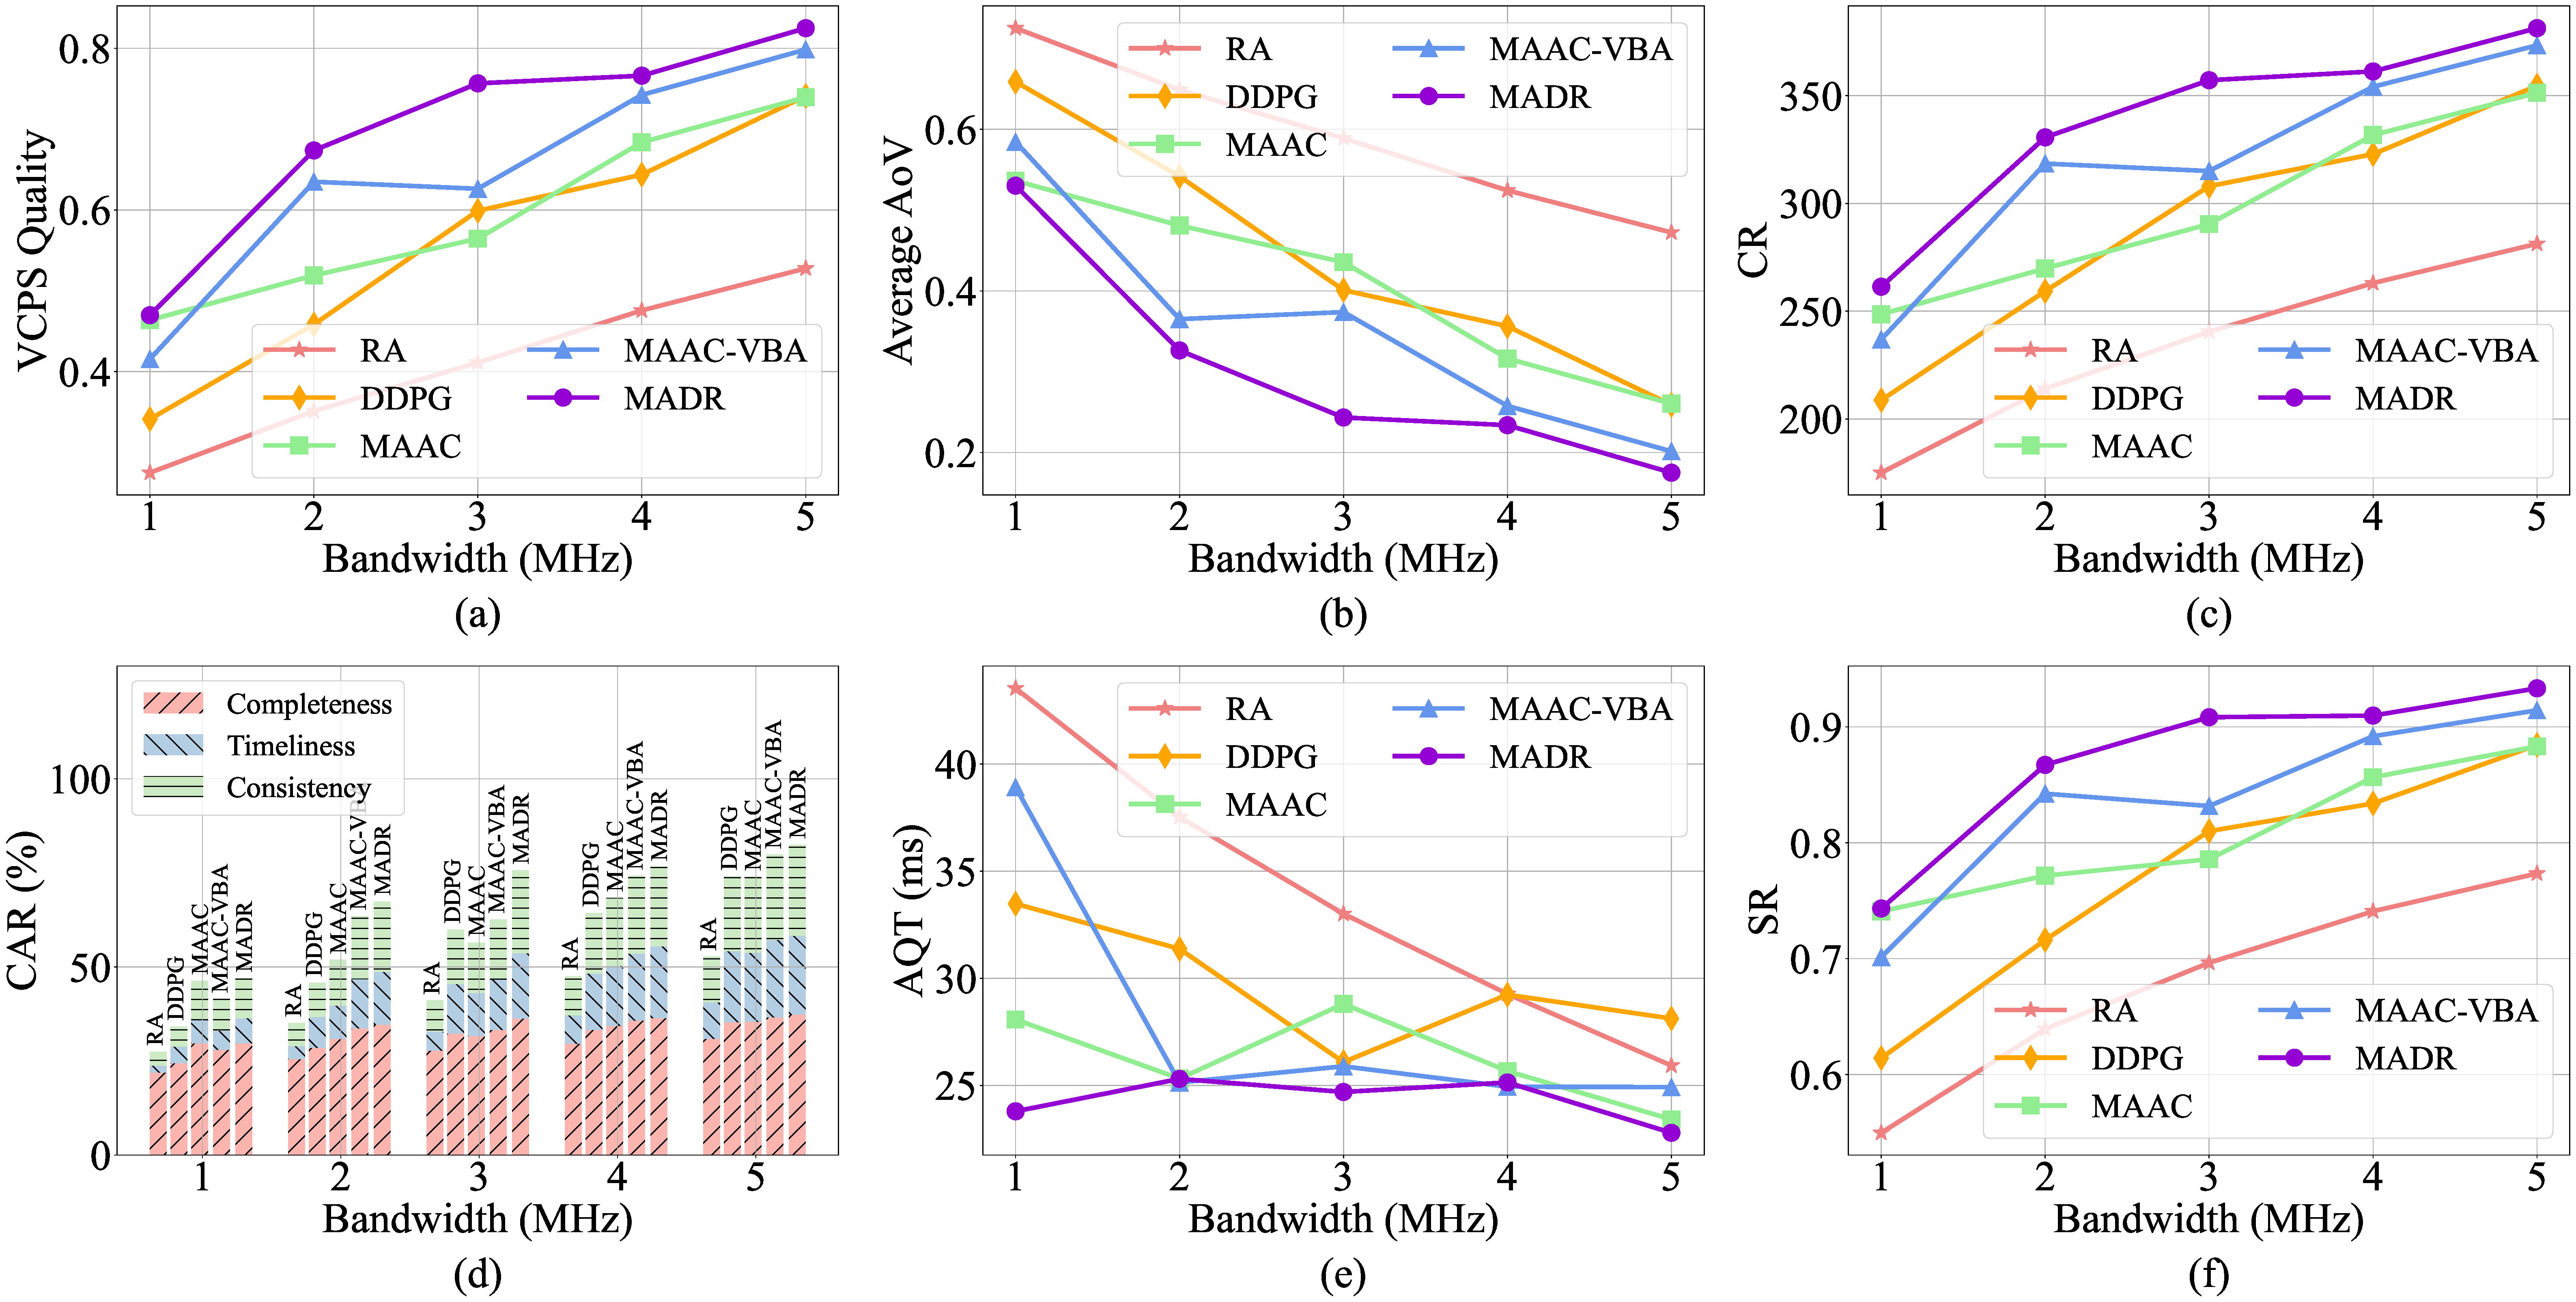
\includegraphics[width=0.9\textwidth]{fig/Fig2-8-different-bandwidths.pdf}
	\end{figure}
\end{textblock*}
\end{center}
}

\only<6-6>{
\begin{center} \englishfont \footnotesize
\begin{textblock*}{\textwidth}(-2.6cm,1.8cm)
{\LARGE{\color{red}\ding{216}}}
\end{textblock*}
\end{center}

\begin{center} \englishfont \footnotesize
\begin{textblock*}{\textwidth}(1cm,3.35cm)
{\LARGE{\color{red}\ding{216}}}
\end{textblock*}
\end{center}

\begin{center} \englishfont \footnotesize
\begin{textblock*}{\textwidth}(5.7cm,1.7cm)
{\LARGE{\color{red}\ding{216}}}
\end{textblock*}
\end{center}

\begin{center} \englishfont \footnotesize
\begin{textblock*}{\textwidth}(0.85cm,6.8cm)
{\LARGE{\color{red}\ding{216}}}
\end{textblock*}
\end{center}

\begin{center} \englishfont \footnotesize
\begin{textblock*}{\textwidth}(5.65cm,4.9cm)
{\LARGE{\color{red}\ding{216}}}
\end{textblock*}
\end{center}
}

\only<7-7>{
\frametitle{\englishfont \underline{实验}:视图需求的影响}
\begin{center} \englishfont \footnotesize
\begin{textblock*}{\textwidth}(1cm,1.8cm)
	\begin{figure}
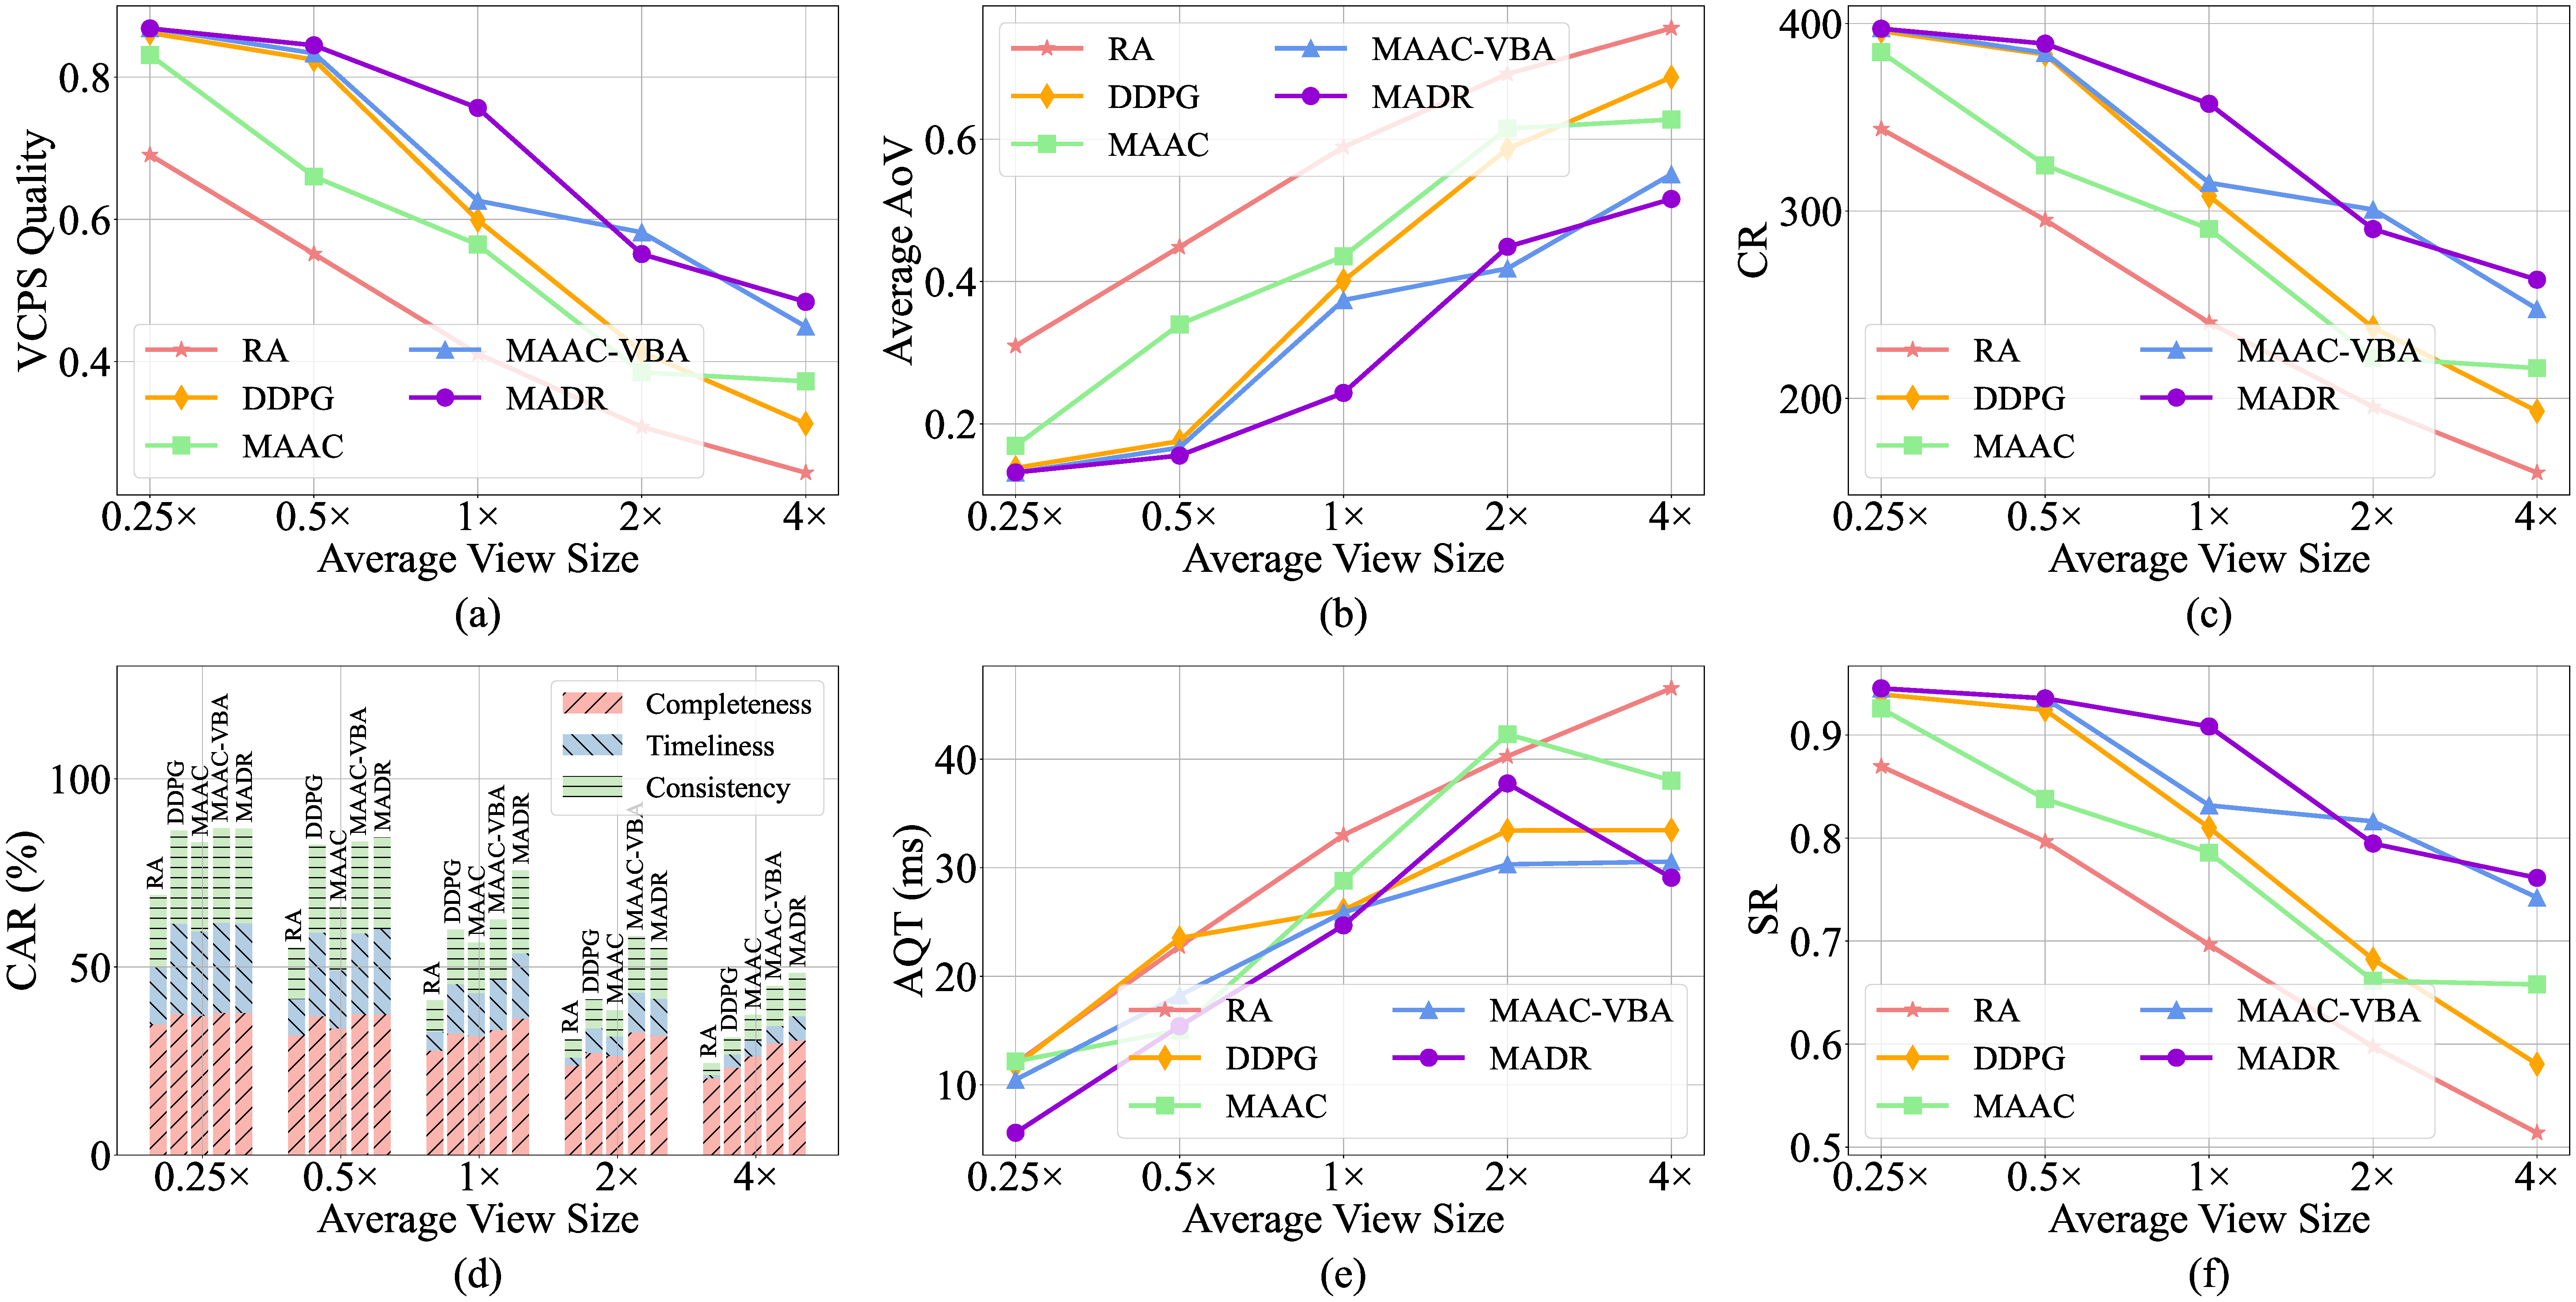
\includegraphics[width=0.9\textwidth]{fig/Fig2-9-different-view-sizes.pdf}
	\end{figure}
\end{textblock*}
\end{center}
}

\only<8-8>{
\frametitle{\englishfont \underline{实验}:视图需求的影响}
\begin{center} \englishfont \footnotesize
\begin{textblock*}{\textwidth}(1cm,1.8cm)
	\begin{figure}
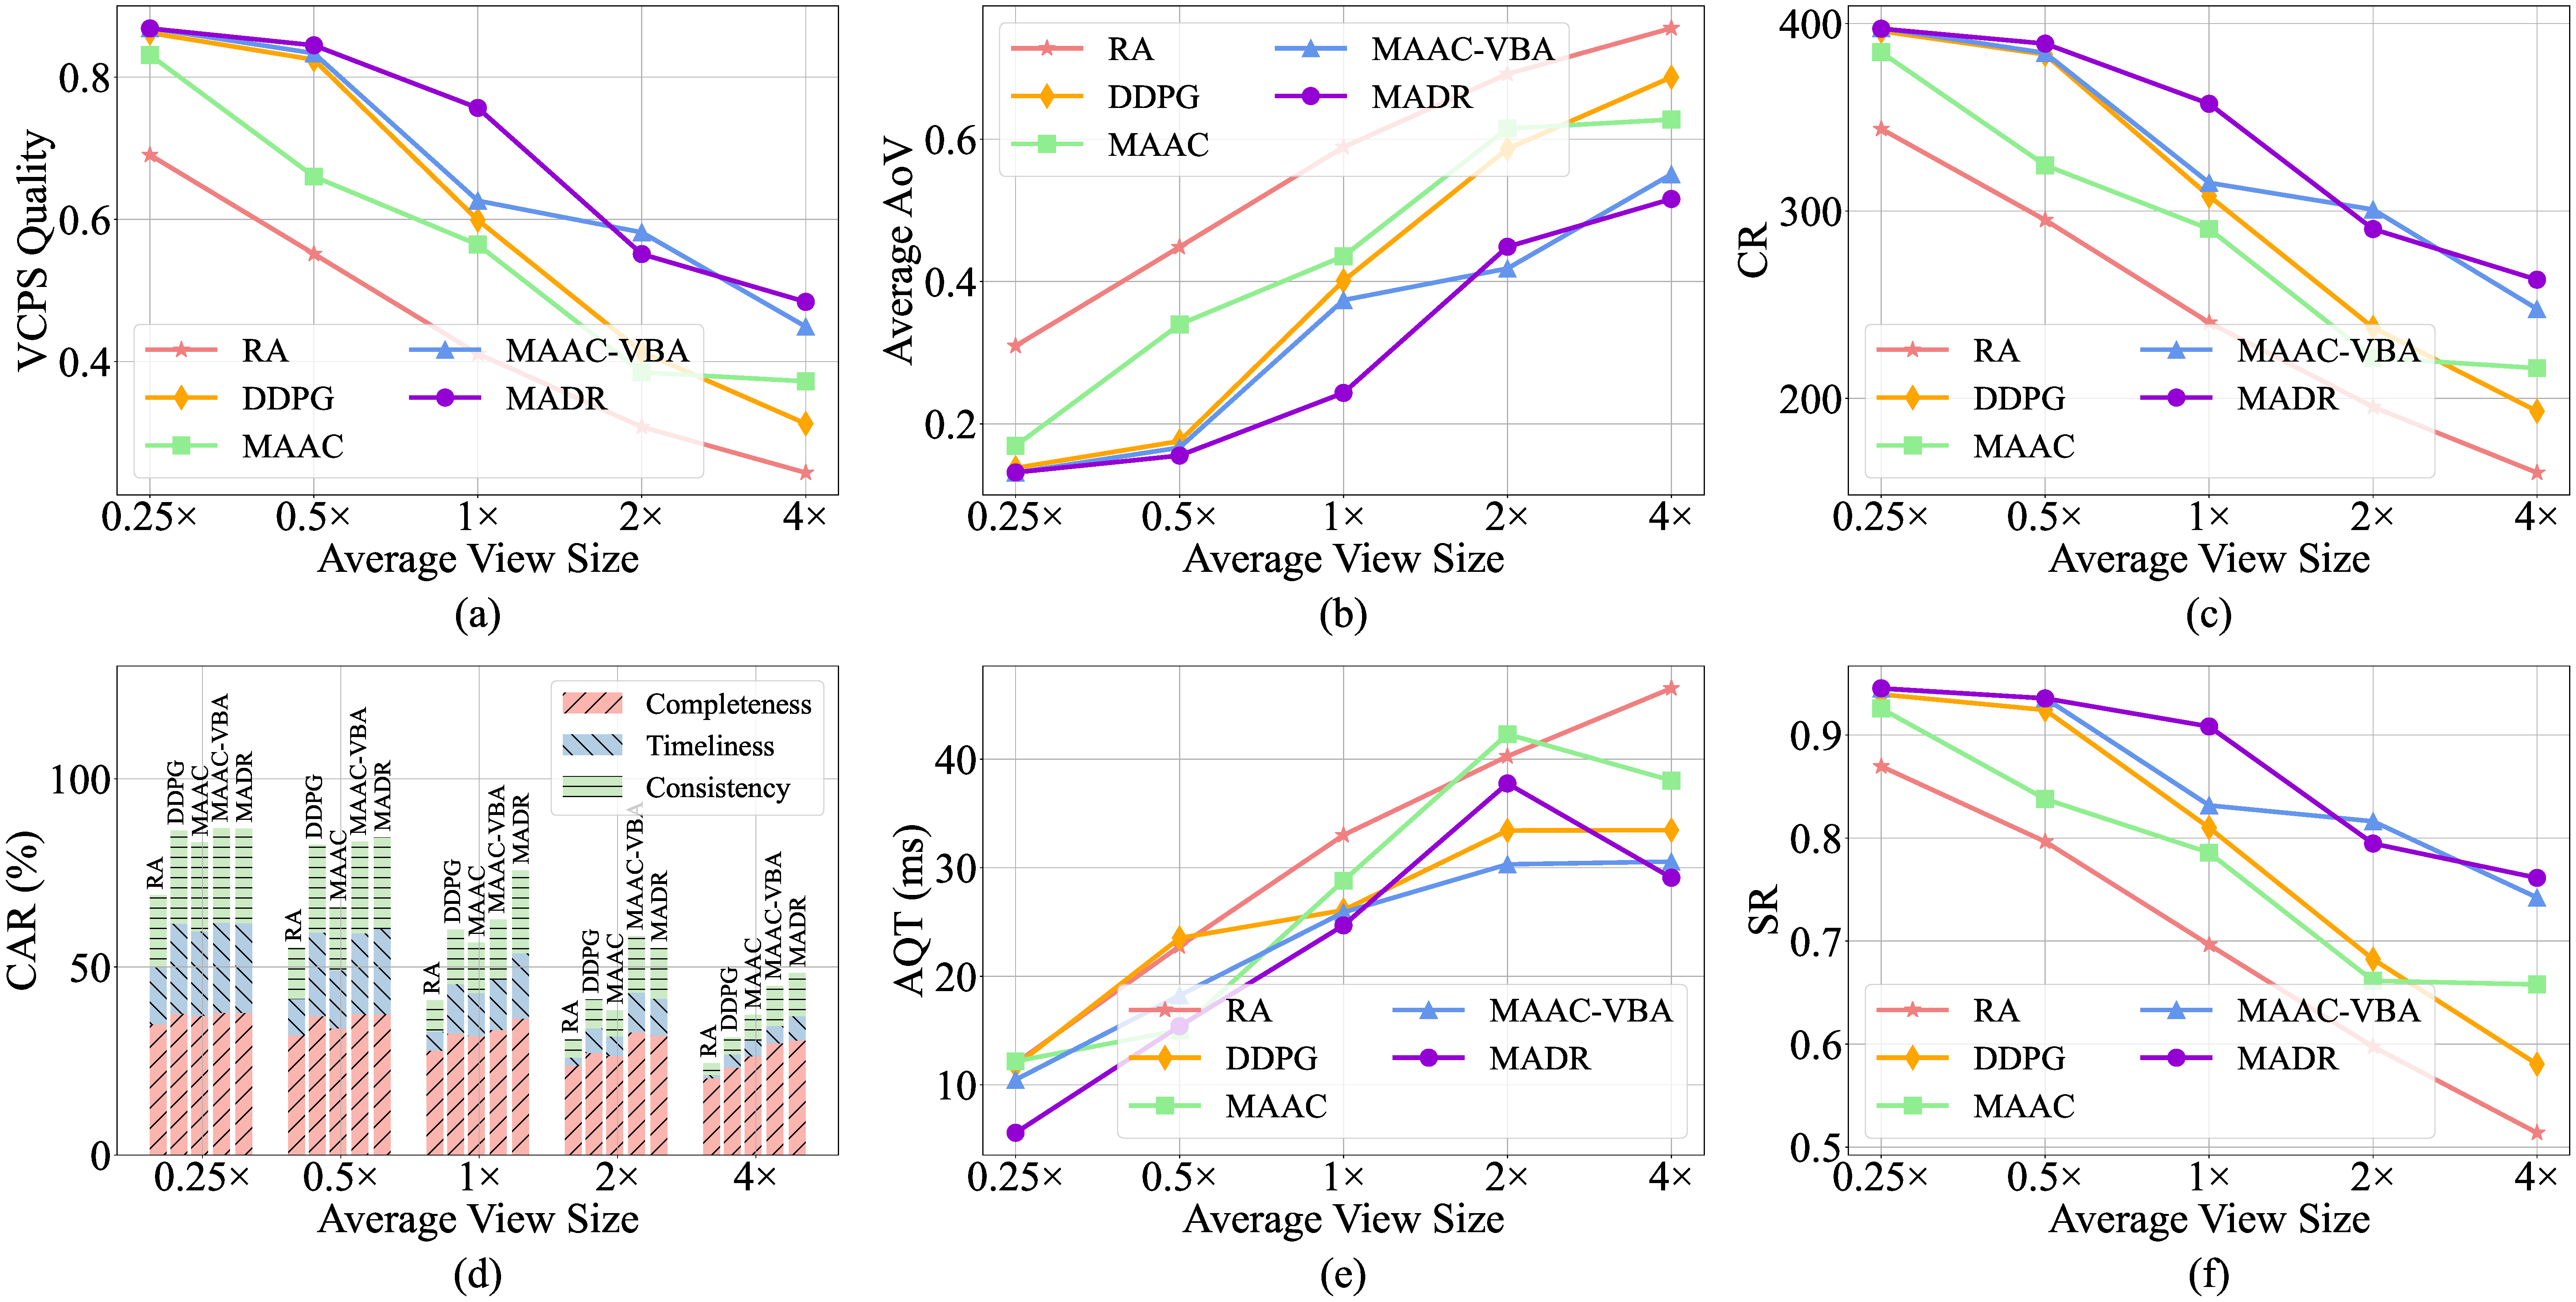
\includegraphics[width=0.9\textwidth]{fig/Fig2-9-different-view-sizes.pdf}
	\end{figure}
\end{textblock*}
\end{center}
}

\only<8-8>{
\begin{center} \englishfont \footnotesize
\begin{textblock*}{\textwidth}(-2.9cm,2cm)
{\LARGE{\color{red}\ding{216}}}
\end{textblock*}
\end{center}

\begin{center} \englishfont \footnotesize
\begin{textblock*}{\textwidth}(1cm,3.35cm)
{\LARGE{\color{red}\ding{216}}}
\end{textblock*}
\end{center}

\begin{center} \englishfont \footnotesize
\begin{textblock*}{\textwidth}(5.5cm,2cm)
{\LARGE{\color{red}\ding{216}}}
\end{textblock*}
\end{center}

\begin{center} \englishfont \footnotesize
\begin{textblock*}{\textwidth}(0.65cm,6.26cm)
{\LARGE{\color{red}\ding{216}}}
\end{textblock*}
\end{center}

\begin{center} \englishfont \footnotesize
\begin{textblock*}{\textwidth}(5.5cm,5cm)
{\LARGE{\color{red}\ding{216}}}
\end{textblock*}
\end{center}
}

\end{overlayarea}
\end{frame}